\documentclass[twoside]{book}

% Packages required by doxygen
\usepackage{fixltx2e}
\usepackage{calc}
\usepackage{doxygen}
\usepackage[export]{adjustbox} % also loads graphicx
\usepackage{graphicx}
\usepackage[utf8]{inputenc}
\usepackage{makeidx}
\usepackage{multicol}
\usepackage{multirow}
\PassOptionsToPackage{warn}{textcomp}
\usepackage{textcomp}
\usepackage[nointegrals]{wasysym}
\usepackage[table]{xcolor}

% Font selection
\usepackage[T1]{fontenc}
\usepackage[scaled=.90]{helvet}
\usepackage{courier}
\usepackage{amssymb}
\usepackage{sectsty}
\renewcommand{\familydefault}{\sfdefault}
\allsectionsfont{%
  \fontseries{bc}\selectfont%
  \color{darkgray}%
}
\renewcommand{\DoxyLabelFont}{%
  \fontseries{bc}\selectfont%
  \color{darkgray}%
}
\newcommand{\+}{\discretionary{\mbox{\scriptsize$\hookleftarrow$}}{}{}}

% Page & text layout
\usepackage{geometry}
\geometry{%
  a4paper,%
  top=2.5cm,%
  bottom=2.5cm,%
  left=2.5cm,%
  right=2.5cm%
}
\tolerance=750
\hfuzz=15pt
\hbadness=750
\setlength{\emergencystretch}{15pt}
\setlength{\parindent}{0cm}
\setlength{\parskip}{3ex plus 2ex minus 2ex}
\makeatletter
\renewcommand{\paragraph}{%
  \@startsection{paragraph}{4}{0ex}{-1.0ex}{1.0ex}{%
    \normalfont\normalsize\bfseries\SS@parafont%
  }%
}
\renewcommand{\subparagraph}{%
  \@startsection{subparagraph}{5}{0ex}{-1.0ex}{1.0ex}{%
    \normalfont\normalsize\bfseries\SS@subparafont%
  }%
}
\makeatother

% Headers & footers
\usepackage{fancyhdr}
\pagestyle{fancyplain}
\fancyhead[LE]{\fancyplain{}{\bfseries\thepage}}
\fancyhead[CE]{\fancyplain{}{}}
\fancyhead[RE]{\fancyplain{}{\bfseries\leftmark}}
\fancyhead[LO]{\fancyplain{}{\bfseries\rightmark}}
\fancyhead[CO]{\fancyplain{}{}}
\fancyhead[RO]{\fancyplain{}{\bfseries\thepage}}
\fancyfoot[LE]{\fancyplain{}{}}
\fancyfoot[CE]{\fancyplain{}{}}
\fancyfoot[RE]{\fancyplain{}{\bfseries\scriptsize Generated by Doxygen }}
\fancyfoot[LO]{\fancyplain{}{\bfseries\scriptsize Generated by Doxygen }}
\fancyfoot[CO]{\fancyplain{}{}}
\fancyfoot[RO]{\fancyplain{}{}}
\renewcommand{\footrulewidth}{0.4pt}
\renewcommand{\chaptermark}[1]{%
  \markboth{#1}{}%
}
\renewcommand{\sectionmark}[1]{%
  \markright{\thesection\ #1}%
}

% Indices & bibliography
\usepackage{natbib}
\usepackage[titles]{tocloft}
\setcounter{tocdepth}{3}
\setcounter{secnumdepth}{5}
\makeindex

% Hyperlinks (required, but should be loaded last)
\usepackage{ifpdf}
\ifpdf
  \usepackage[pdftex,pagebackref=true]{hyperref}
\else
  \usepackage[ps2pdf,pagebackref=true]{hyperref}
\fi
\hypersetup{%
  colorlinks=true,%
  linkcolor=blue,%
  citecolor=blue,%
  unicode%
}

% Custom commands
\newcommand{\clearemptydoublepage}{%
  \newpage{\pagestyle{empty}\cleardoublepage}%
}

\usepackage{caption}
\captionsetup{labelsep=space,justification=centering,font={bf},singlelinecheck=off,skip=4pt,position=top}

%===== C O N T E N T S =====

\begin{document}

% Titlepage & ToC
\hypersetup{pageanchor=false,
             bookmarksnumbered=true,
             pdfencoding=unicode
            }
\pagenumbering{alph}
\begin{titlepage}
\vspace*{7cm}
\begin{center}%
{\Large Angry Space }\\
\vspace*{1cm}
{\large Generated by Doxygen 1.8.14}\\
\end{center}
\end{titlepage}
\clearemptydoublepage
\pagenumbering{roman}
\tableofcontents
\clearemptydoublepage
\pagenumbering{arabic}
\hypersetup{pageanchor=true}

%--- Begin generated contents ---
\chapter{Hierarchical Index}
\section{Class Hierarchy}
This inheritance list is sorted roughly, but not completely, alphabetically\+:\begin{DoxyCompactList}
\item Mono\+Behaviour\begin{DoxyCompactList}
\item \contentsline{section}{A\+I\+Enemy}{\pageref{class_a_i_enemy}}{}
\item \contentsline{section}{Asteroid\+Attributes}{\pageref{class_asteroid_attributes}}{}
\item \contentsline{section}{Asteroid\+Generator}{\pageref{class_asteroid_generator}}{}
\item \contentsline{section}{Bonuses\+Controller}{\pageref{class_bonuses_controller}}{}
\item \contentsline{section}{Bonus\+Movement}{\pageref{class_bonus_movement}}{}
\item \contentsline{section}{Bullet\+Movement}{\pageref{class_bullet_movement}}{}
\item \contentsline{section}{Calculate\+Screen\+Bounds}{\pageref{class_calculate_screen_bounds}}{}
\item \contentsline{section}{Change\+Scene\+Button}{\pageref{class_change_scene_button}}{}
\item \contentsline{section}{Click\+Buttons}{\pageref{class_click_buttons}}{}
\item \contentsline{section}{Collision\+Bullet}{\pageref{class_collision_bullet}}{}
\item \contentsline{section}{Game\+Over}{\pageref{class_game_over}}{}
\item \contentsline{section}{Instantiate\+Bullet}{\pageref{class_instantiate_bullet}}{}
\item \contentsline{section}{Move}{\pageref{class_move}}{}
\item \contentsline{section}{Pause\+Game}{\pageref{class_pause_game}}{}
\item \contentsline{section}{Place\+Score\+Bars}{\pageref{class_place_score_bars}}{}
\item \contentsline{section}{Planet\+Lifes\+Controller}{\pageref{class_planet_lifes_controller}}{}
\item \contentsline{section}{Play\+Again}{\pageref{class_play_again}}{}
\item \contentsline{section}{Player\+Attributes}{\pageref{class_player_attributes}}{}
\item \contentsline{section}{Player\+Chooser}{\pageref{class_player_chooser}}{}
\item \contentsline{section}{Player\+Key\+Controller}{\pageref{class_player_key_controller}}{}
\item \contentsline{section}{Quit\+Game}{\pageref{class_quit_game}}{}
\item \contentsline{section}{rotate}{\pageref{classrotate}}{}
\item \contentsline{section}{Start\+Playing\+Scene}{\pageref{class_start_playing_scene}}{}
\item \contentsline{section}{Text\+Manager}{\pageref{class_text_manager}}{}
\end{DoxyCompactList}
\end{DoxyCompactList}

\chapter{Class Index}
\section{Class List}
Here are the classes, structs, unions and interfaces with brief descriptions\+:\begin{DoxyCompactList}
\item\contentsline{section}{\mbox{\hyperlink{class_a_i_enemy}{A\+I\+Enemy}} \\*AI enemy class }{\pageref{class_a_i_enemy}}{}
\item\contentsline{section}{\mbox{\hyperlink{class_asteroid_attributes}{Asteroid\+Attributes}} \\*Class representing asteroid attributes. }{\pageref{class_asteroid_attributes}}{}
\item\contentsline{section}{\mbox{\hyperlink{class_asteroid_generator}{Asteroid\+Generator}} \\*Asteroid generator. }{\pageref{class_asteroid_generator}}{}
\item\contentsline{section}{\mbox{\hyperlink{class_bonuses_controller}{Bonuses\+Controller}} \\*Class responsible for controlling bonuses. }{\pageref{class_bonuses_controller}}{}
\item\contentsline{section}{\mbox{\hyperlink{class_bonus_movement}{Bonus\+Movement}} \\*Class responsible for movement of bonus (side, speed). }{\pageref{class_bonus_movement}}{}
\item\contentsline{section}{\mbox{\hyperlink{class_bullet_movement}{Bullet\+Movement}} \\*The movement of the bullet, including parts where it rotates around a planet. }{\pageref{class_bullet_movement}}{}
\item\contentsline{section}{\mbox{\hyperlink{class_calculate_screen_bounds}{Calculate\+Screen\+Bounds}} \\*Class responsible for calculating screen bounds, depending on resolution etc. }{\pageref{class_calculate_screen_bounds}}{}
\item\contentsline{section}{\mbox{\hyperlink{class_change_scene_button}{Change\+Scene\+Button}} \\*Class responsible for changing the scenes. }{\pageref{class_change_scene_button}}{}
\item\contentsline{section}{\mbox{\hyperlink{class_click_buttons}{Click\+Buttons}} \\*Clas responsible for reacting to clicking buttons. }{\pageref{class_click_buttons}}{}
\item\contentsline{section}{\mbox{\hyperlink{class_collision_bullet}{Collision\+Bullet}} \\*Collision player with bullet manager }{\pageref{class_collision_bullet}}{}
\item\contentsline{section}{\mbox{\hyperlink{class_game_over}{Game\+Over}} \\*Class responsible of showing \char`\"{}\+Game Over\char`\"{} canvas if one player looses. }{\pageref{class_game_over}}{}
\item\contentsline{section}{\mbox{\hyperlink{class_instantiate_bullet}{Instantiate\+Bullet}} \\*Instantiate bullet. }{\pageref{class_instantiate_bullet}}{}
\item\contentsline{section}{\mbox{\hyperlink{class_move}{Move}} \\*Class responsible for player movement. }{\pageref{class_move}}{}
\item\contentsline{section}{\mbox{\hyperlink{class_pause_game}{Pause\+Game}} \\*Class responsible of pausing the game. }{\pageref{class_pause_game}}{}
\item\contentsline{section}{\mbox{\hyperlink{class_place_score_bars}{Place\+Score\+Bars}} \\*Class responsible for placing score bars. }{\pageref{class_place_score_bars}}{}
\item\contentsline{section}{\mbox{\hyperlink{class_planet_lifes_controller}{Planet\+Lifes\+Controller}} \\*Class to control planet lifes and show explosion effect after it dies. }{\pageref{class_planet_lifes_controller}}{}
\item\contentsline{section}{\mbox{\hyperlink{class_play_again}{Play\+Again}} \\*Class responsible for playing the scene again. }{\pageref{class_play_again}}{}
\item\contentsline{section}{\mbox{\hyperlink{class_player_attributes}{Player\+Attributes}} \\*Player attributes, like speed, rate of fire, ... }{\pageref{class_player_attributes}}{}
\item\contentsline{section}{\mbox{\hyperlink{class_player_chooser}{Player\+Chooser}} \\*Class responsible for settig proper fields after user chooses playing mode (one or two players). }{\pageref{class_player_chooser}}{}
\item\contentsline{section}{\mbox{\hyperlink{class_player_key_controller}{Player\+Key\+Controller}} \\*Player key controller, after pushing the button, update position of the player }{\pageref{class_player_key_controller}}{}
\item\contentsline{section}{\mbox{\hyperlink{class_quit_game}{Quit\+Game}} \\*Class responsible for quiting the game. }{\pageref{class_quit_game}}{}
\item\contentsline{section}{\mbox{\hyperlink{classrotate}{rotate}} \\*Class responsible of rotation. }{\pageref{classrotate}}{}
\item\contentsline{section}{\mbox{\hyperlink{class_start_playing_scene}{Start\+Playing\+Scene}} \\*Class responsible for starting playing the game. }{\pageref{class_start_playing_scene}}{}
\item\contentsline{section}{\mbox{\hyperlink{class_text_manager}{Text\+Manager}} \\*Player\textquotesingle{}s text manu manager }{\pageref{class_text_manager}}{}
\end{DoxyCompactList}

\chapter{Class Documentation}
\hypertarget{class_a_i_enemy}{}\section{A\+I\+Enemy Class Reference}
\label{class_a_i_enemy}\index{A\+I\+Enemy@{A\+I\+Enemy}}


AI enemy class  


Inheritance diagram for A\+I\+Enemy\+:\begin{figure}[H]
\begin{center}
\leavevmode
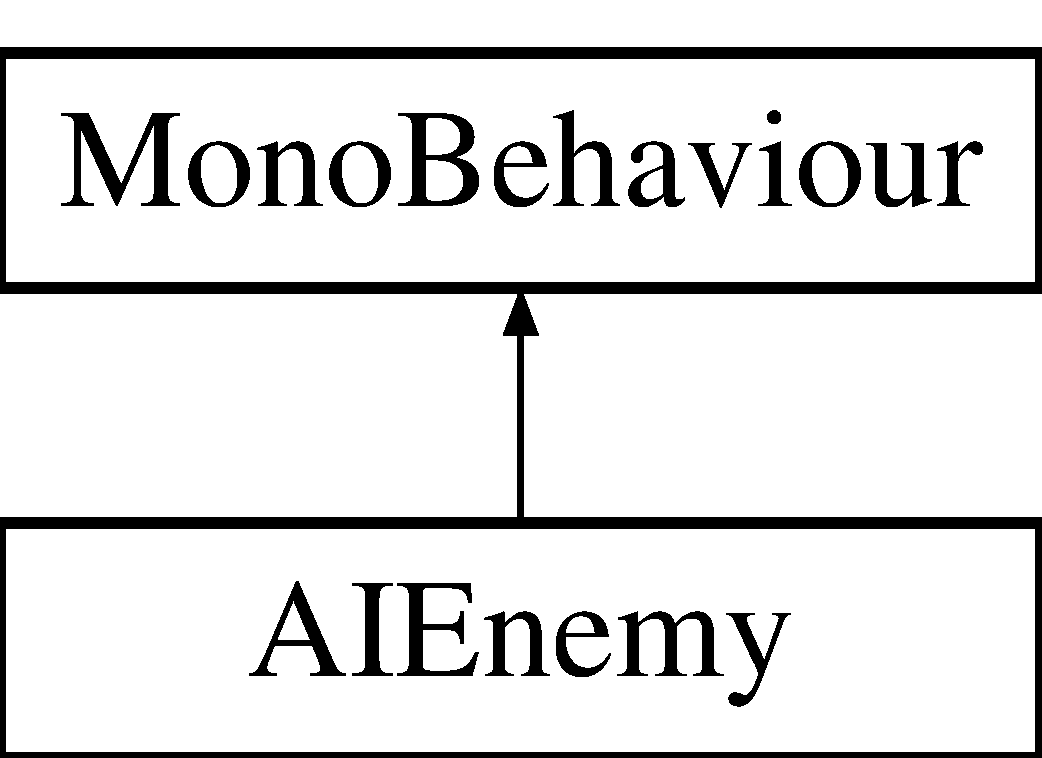
\includegraphics[height=2.000000cm]{class_a_i_enemy}
\end{center}
\end{figure}
\subsection*{Public Attributes}
\begin{DoxyCompactItemize}
\item 
int \mbox{\hyperlink{class_a_i_enemy_a4514cc12da817389aefe66b88929422a}{chance\+To\+Shoot}}
\begin{DoxyCompactList}\small\item\em The chance to shoot. \end{DoxyCompactList}\end{DoxyCompactItemize}


\subsection{Detailed Description}
AI enemy class 



\subsection{Member Data Documentation}
\mbox{\Hypertarget{class_a_i_enemy_a4514cc12da817389aefe66b88929422a}\label{class_a_i_enemy_a4514cc12da817389aefe66b88929422a}} 
\index{A\+I\+Enemy@{A\+I\+Enemy}!chance\+To\+Shoot@{chance\+To\+Shoot}}
\index{chance\+To\+Shoot@{chance\+To\+Shoot}!A\+I\+Enemy@{A\+I\+Enemy}}
\subsubsection{\texorpdfstring{chance\+To\+Shoot}{chanceToShoot}}
{\footnotesize\ttfamily int A\+I\+Enemy.\+chance\+To\+Shoot}



The chance to shoot. 



The documentation for this class was generated from the following file\+:\begin{DoxyCompactItemize}
\item 
Player/A\+I\+Enemy.\+cs\end{DoxyCompactItemize}

\hypertarget{class_asteroid_attributes}{}\section{Asteroid\+Attributes Class Reference}
\label{class_asteroid_attributes}\index{Asteroid\+Attributes@{Asteroid\+Attributes}}


Class representing asteroid attributes.  


Inheritance diagram for Asteroid\+Attributes\+:\begin{figure}[H]
\begin{center}
\leavevmode
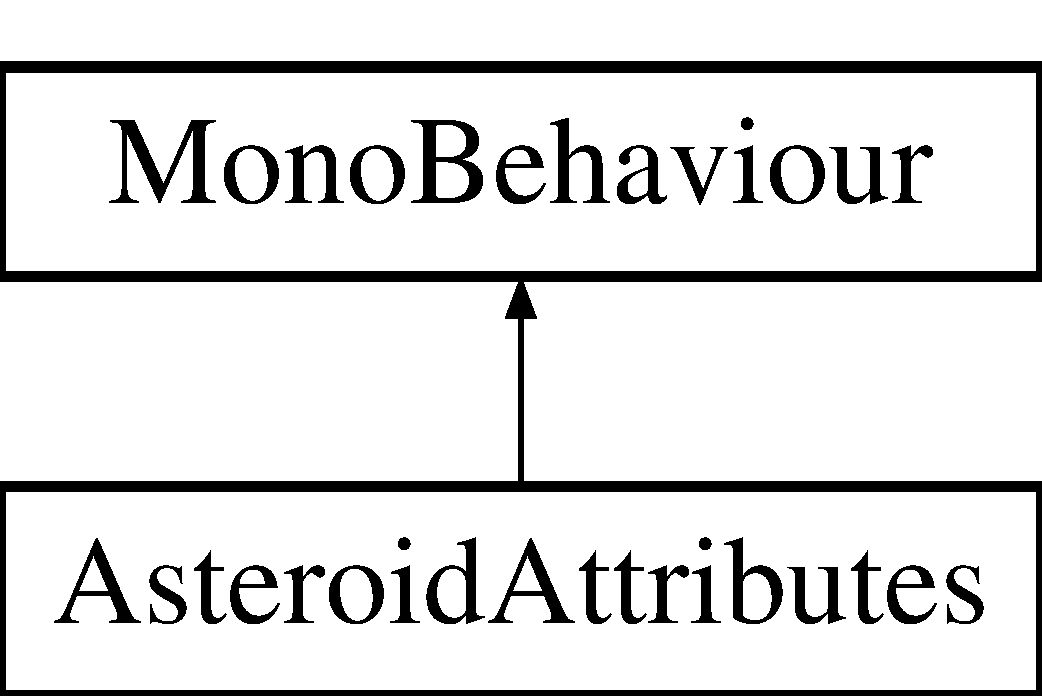
\includegraphics[height=2.000000cm]{class_asteroid_attributes}
\end{center}
\end{figure}
\subsection*{Public Attributes}
\begin{DoxyCompactItemize}
\item 
int \mbox{\hyperlink{class_asteroid_attributes_a671f2c91e2ad27a1f1d45346ec8dcd22}{mass}}
\begin{DoxyCompactList}\small\item\em Mass of the asteroid. \end{DoxyCompactList}\item 
int \mbox{\hyperlink{class_asteroid_attributes_a8cc9267ef0f5534260f7ccb7c16c04ca}{radius}}
\begin{DoxyCompactList}\small\item\em Radius of the asteroid collider. \end{DoxyCompactList}\item 
Game\+Object \mbox{\hyperlink{class_asteroid_attributes_a25d09f5bc06ec1aa4761fe4ec30eebca}{collider\+Sprite}}
\begin{DoxyCompactList}\small\item\em The collider sprite. \end{DoxyCompactList}\end{DoxyCompactItemize}
\subsection*{Private Member Functions}
\begin{DoxyCompactItemize}
\item 
void \mbox{\hyperlink{class_asteroid_attributes_a61f24598b995b4629d3426dabb7cfa6a}{Start}} ()
\begin{DoxyCompactList}\small\item\em Sets radius and mass to the asteroid components. \end{DoxyCompactList}\end{DoxyCompactItemize}


\subsection{Detailed Description}
Class representing asteroid attributes. 



\subsection{Member Function Documentation}
\mbox{\Hypertarget{class_asteroid_attributes_a61f24598b995b4629d3426dabb7cfa6a}\label{class_asteroid_attributes_a61f24598b995b4629d3426dabb7cfa6a}} 
\index{Asteroid\+Attributes@{Asteroid\+Attributes}!Start@{Start}}
\index{Start@{Start}!Asteroid\+Attributes@{Asteroid\+Attributes}}
\subsubsection{\texorpdfstring{Start()}{Start()}}
{\footnotesize\ttfamily void Asteroid\+Attributes.\+Start (\begin{DoxyParamCaption}{ }\end{DoxyParamCaption})\hspace{0.3cm}{\ttfamily [private]}}



Sets radius and mass to the asteroid components. 



\subsection{Member Data Documentation}
\mbox{\Hypertarget{class_asteroid_attributes_a25d09f5bc06ec1aa4761fe4ec30eebca}\label{class_asteroid_attributes_a25d09f5bc06ec1aa4761fe4ec30eebca}} 
\index{Asteroid\+Attributes@{Asteroid\+Attributes}!collider\+Sprite@{collider\+Sprite}}
\index{collider\+Sprite@{collider\+Sprite}!Asteroid\+Attributes@{Asteroid\+Attributes}}
\subsubsection{\texorpdfstring{collider\+Sprite}{colliderSprite}}
{\footnotesize\ttfamily Game\+Object Asteroid\+Attributes.\+collider\+Sprite}



The collider sprite. 

\mbox{\Hypertarget{class_asteroid_attributes_a671f2c91e2ad27a1f1d45346ec8dcd22}\label{class_asteroid_attributes_a671f2c91e2ad27a1f1d45346ec8dcd22}} 
\index{Asteroid\+Attributes@{Asteroid\+Attributes}!mass@{mass}}
\index{mass@{mass}!Asteroid\+Attributes@{Asteroid\+Attributes}}
\subsubsection{\texorpdfstring{mass}{mass}}
{\footnotesize\ttfamily int Asteroid\+Attributes.\+mass}



Mass of the asteroid. 

\mbox{\Hypertarget{class_asteroid_attributes_a8cc9267ef0f5534260f7ccb7c16c04ca}\label{class_asteroid_attributes_a8cc9267ef0f5534260f7ccb7c16c04ca}} 
\index{Asteroid\+Attributes@{Asteroid\+Attributes}!radius@{radius}}
\index{radius@{radius}!Asteroid\+Attributes@{Asteroid\+Attributes}}
\subsubsection{\texorpdfstring{radius}{radius}}
{\footnotesize\ttfamily int Asteroid\+Attributes.\+radius}



Radius of the asteroid collider. 



The documentation for this class was generated from the following file\+:\begin{DoxyCompactItemize}
\item 
Asteroid\+Attributes.\+cs\end{DoxyCompactItemize}

\hypertarget{class_asteroid_generator}{}\section{Asteroid\+Generator Class Reference}
\label{class_asteroid_generator}\index{Asteroid\+Generator@{Asteroid\+Generator}}


Asteroid generator.  


Inheritance diagram for Asteroid\+Generator\+:\begin{figure}[H]
\begin{center}
\leavevmode
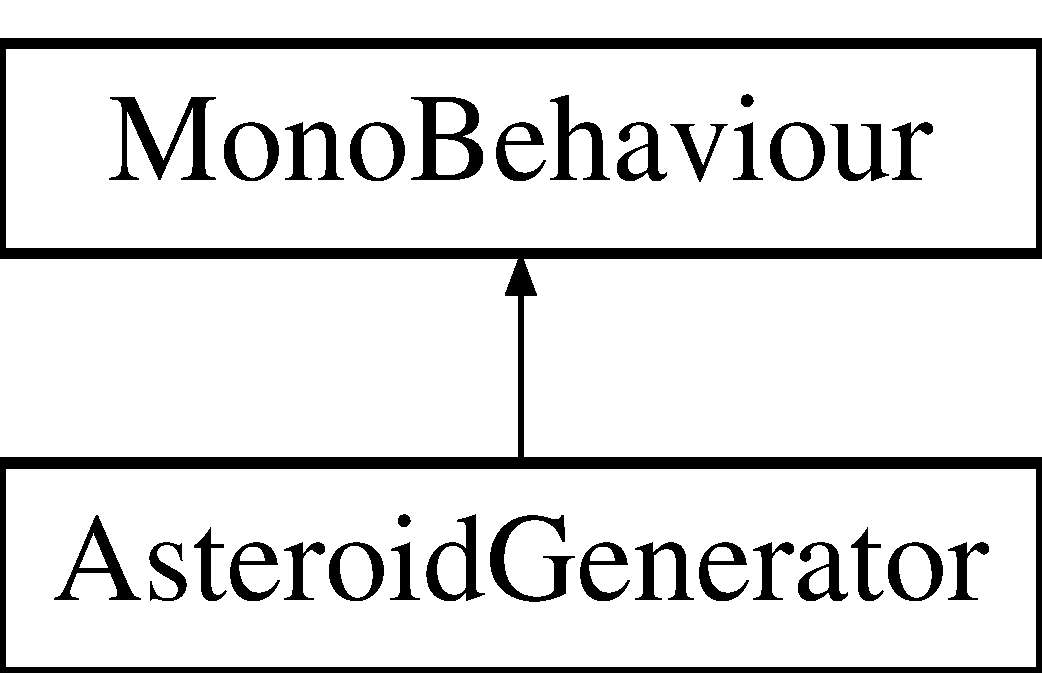
\includegraphics[height=2.000000cm]{class_asteroid_generator}
\end{center}
\end{figure}
\subsection*{Public Attributes}
\begin{DoxyCompactItemize}
\item 
int \mbox{\hyperlink{class_asteroid_generator_a4cc51b71a8eb59ad4fa0a58b1ab2fdbc}{Number\+Of\+Asteroids}}
\begin{DoxyCompactList}\small\item\em The number of asteroids. \end{DoxyCompactList}\item 
List$<$ Game\+Object $>$ \mbox{\hyperlink{class_asteroid_generator_a96adffc17fece791d1735c8ffd72cd43}{Asteroid\+List}}
\begin{DoxyCompactList}\small\item\em The asteroid list. \end{DoxyCompactList}\item 
List$<$ Game\+Object $>$ \mbox{\hyperlink{class_asteroid_generator_a3547304e3d1a3777f6d996e7f6c409de}{added\+Asteroid\+List}} = new List$<$Game\+Object$>$ ()
\begin{DoxyCompactList}\small\item\em List of already created asteroids. \end{DoxyCompactList}\item 
int \mbox{\hyperlink{class_asteroid_generator_ac4789385fb5a11f27cf743ddf1e32f93}{Min\+Mass}}
\begin{DoxyCompactList}\small\item\em The minimum mass. \end{DoxyCompactList}\item 
int \mbox{\hyperlink{class_asteroid_generator_aaa0eb57c660f14898c0c7b196293584a}{Max\+Mass}}
\begin{DoxyCompactList}\small\item\em The max mass. \end{DoxyCompactList}\item 
int \mbox{\hyperlink{class_asteroid_generator_a7bbc470dbc92203ced647f45cf557940}{Min\+Radius}}
\begin{DoxyCompactList}\small\item\em The minimum radius. \end{DoxyCompactList}\item 
int \mbox{\hyperlink{class_asteroid_generator_a5e008980325a1f5b6faa04a8b44fdc3e}{Max\+Radius}}
\begin{DoxyCompactList}\small\item\em The max radius. \end{DoxyCompactList}\item 
Game\+Object \mbox{\hyperlink{class_asteroid_generator_ab4e16ac73ae5fc15af5704ad3e6f8bc5}{collider\+Sprite}}
\begin{DoxyCompactList}\small\item\em The collider sprite. Gameobject representing every planet\textquotesingle{}s collider. \end{DoxyCompactList}\end{DoxyCompactItemize}


\subsection{Detailed Description}
Asteroid generator. 



\subsection{Member Data Documentation}
\mbox{\Hypertarget{class_asteroid_generator_a3547304e3d1a3777f6d996e7f6c409de}\label{class_asteroid_generator_a3547304e3d1a3777f6d996e7f6c409de}} 
\index{Asteroid\+Generator@{Asteroid\+Generator}!added\+Asteroid\+List@{added\+Asteroid\+List}}
\index{added\+Asteroid\+List@{added\+Asteroid\+List}!Asteroid\+Generator@{Asteroid\+Generator}}
\subsubsection{\texorpdfstring{added\+Asteroid\+List}{addedAsteroidList}}
{\footnotesize\ttfamily List$<$Game\+Object$>$ Asteroid\+Generator.\+added\+Asteroid\+List = new List$<$Game\+Object$>$ ()}



List of already created asteroids. 

\mbox{\Hypertarget{class_asteroid_generator_a96adffc17fece791d1735c8ffd72cd43}\label{class_asteroid_generator_a96adffc17fece791d1735c8ffd72cd43}} 
\index{Asteroid\+Generator@{Asteroid\+Generator}!Asteroid\+List@{Asteroid\+List}}
\index{Asteroid\+List@{Asteroid\+List}!Asteroid\+Generator@{Asteroid\+Generator}}
\subsubsection{\texorpdfstring{Asteroid\+List}{AsteroidList}}
{\footnotesize\ttfamily List$<$Game\+Object$>$ Asteroid\+Generator.\+Asteroid\+List}



The asteroid list. 

\mbox{\Hypertarget{class_asteroid_generator_ab4e16ac73ae5fc15af5704ad3e6f8bc5}\label{class_asteroid_generator_ab4e16ac73ae5fc15af5704ad3e6f8bc5}} 
\index{Asteroid\+Generator@{Asteroid\+Generator}!collider\+Sprite@{collider\+Sprite}}
\index{collider\+Sprite@{collider\+Sprite}!Asteroid\+Generator@{Asteroid\+Generator}}
\subsubsection{\texorpdfstring{collider\+Sprite}{colliderSprite}}
{\footnotesize\ttfamily Game\+Object Asteroid\+Generator.\+collider\+Sprite}



The collider sprite. Gameobject representing every planet\textquotesingle{}s collider. 

\mbox{\Hypertarget{class_asteroid_generator_aaa0eb57c660f14898c0c7b196293584a}\label{class_asteroid_generator_aaa0eb57c660f14898c0c7b196293584a}} 
\index{Asteroid\+Generator@{Asteroid\+Generator}!Max\+Mass@{Max\+Mass}}
\index{Max\+Mass@{Max\+Mass}!Asteroid\+Generator@{Asteroid\+Generator}}
\subsubsection{\texorpdfstring{Max\+Mass}{MaxMass}}
{\footnotesize\ttfamily int Asteroid\+Generator.\+Max\+Mass}



The max mass. 

\mbox{\Hypertarget{class_asteroid_generator_a5e008980325a1f5b6faa04a8b44fdc3e}\label{class_asteroid_generator_a5e008980325a1f5b6faa04a8b44fdc3e}} 
\index{Asteroid\+Generator@{Asteroid\+Generator}!Max\+Radius@{Max\+Radius}}
\index{Max\+Radius@{Max\+Radius}!Asteroid\+Generator@{Asteroid\+Generator}}
\subsubsection{\texorpdfstring{Max\+Radius}{MaxRadius}}
{\footnotesize\ttfamily int Asteroid\+Generator.\+Max\+Radius}



The max radius. 

\mbox{\Hypertarget{class_asteroid_generator_ac4789385fb5a11f27cf743ddf1e32f93}\label{class_asteroid_generator_ac4789385fb5a11f27cf743ddf1e32f93}} 
\index{Asteroid\+Generator@{Asteroid\+Generator}!Min\+Mass@{Min\+Mass}}
\index{Min\+Mass@{Min\+Mass}!Asteroid\+Generator@{Asteroid\+Generator}}
\subsubsection{\texorpdfstring{Min\+Mass}{MinMass}}
{\footnotesize\ttfamily int Asteroid\+Generator.\+Min\+Mass}



The minimum mass. 

\mbox{\Hypertarget{class_asteroid_generator_a7bbc470dbc92203ced647f45cf557940}\label{class_asteroid_generator_a7bbc470dbc92203ced647f45cf557940}} 
\index{Asteroid\+Generator@{Asteroid\+Generator}!Min\+Radius@{Min\+Radius}}
\index{Min\+Radius@{Min\+Radius}!Asteroid\+Generator@{Asteroid\+Generator}}
\subsubsection{\texorpdfstring{Min\+Radius}{MinRadius}}
{\footnotesize\ttfamily int Asteroid\+Generator.\+Min\+Radius}



The minimum radius. 

\mbox{\Hypertarget{class_asteroid_generator_a4cc51b71a8eb59ad4fa0a58b1ab2fdbc}\label{class_asteroid_generator_a4cc51b71a8eb59ad4fa0a58b1ab2fdbc}} 
\index{Asteroid\+Generator@{Asteroid\+Generator}!Number\+Of\+Asteroids@{Number\+Of\+Asteroids}}
\index{Number\+Of\+Asteroids@{Number\+Of\+Asteroids}!Asteroid\+Generator@{Asteroid\+Generator}}
\subsubsection{\texorpdfstring{Number\+Of\+Asteroids}{NumberOfAsteroids}}
{\footnotesize\ttfamily int Asteroid\+Generator.\+Number\+Of\+Asteroids}



The number of asteroids. 



The documentation for this class was generated from the following file\+:\begin{DoxyCompactItemize}
\item 
Asteroid\+Generator.\+cs\end{DoxyCompactItemize}

\hypertarget{class_bonuses_controller}{}\section{Bonuses\+Controller Class Reference}
\label{class_bonuses_controller}\index{Bonuses\+Controller@{Bonuses\+Controller}}


Class responsible for controlling bonuses.  


Inheritance diagram for Bonuses\+Controller\+:\begin{figure}[H]
\begin{center}
\leavevmode
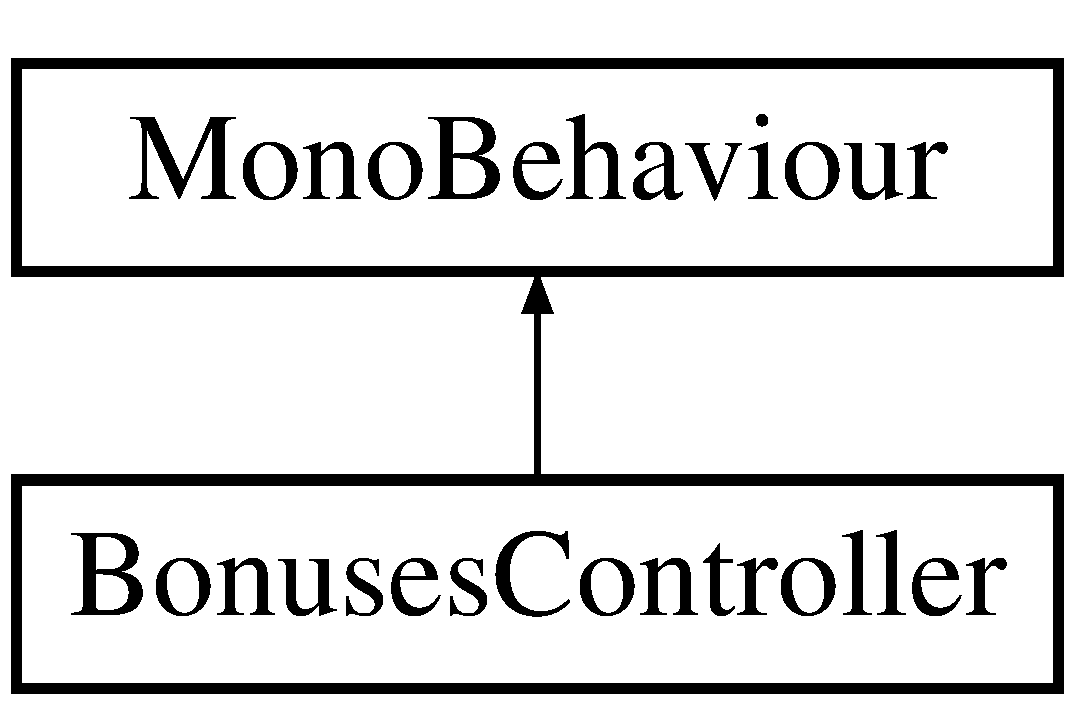
\includegraphics[height=2.000000cm]{class_bonuses_controller}
\end{center}
\end{figure}
\subsection*{Public Attributes}
\begin{DoxyCompactItemize}
\item 
int \mbox{\hyperlink{class_bonuses_controller_a01de764707e69ec225d62563fc683cd5}{bonus\+Rate}}
\begin{DoxyCompactList}\small\item\em Chance that there will be created bonus in asteroid\textquotesingle{}s place. \end{DoxyCompactList}\item 
int \mbox{\hyperlink{class_bonuses_controller_a5832f0f45d1b3f889da0fd3eafcfd054}{bonuses\+Number}}
\begin{DoxyCompactList}\small\item\em Number of possible bonuses kinds. \end{DoxyCompactList}\item 
List$<$ Game\+Object $>$ \mbox{\hyperlink{class_bonuses_controller_adb877f81531327caebb69f2f2aa292f1}{bonuses}}
\begin{DoxyCompactList}\small\item\em List of possible bonuses kinds. \end{DoxyCompactList}\item 
int \mbox{\hyperlink{class_bonuses_controller_a14eaa862f70cb157749cb0978ef5bd96}{planet\+Lifes}}
\begin{DoxyCompactList}\small\item\em Planet lifes. When equals to zero, the planet will be destroyed and with some probability there should appear bonus in planet\textquotesingle{}s place. \end{DoxyCompactList}\end{DoxyCompactItemize}


\subsection{Detailed Description}
Class responsible for controlling bonuses. 



\subsection{Member Data Documentation}
\mbox{\Hypertarget{class_bonuses_controller_adb877f81531327caebb69f2f2aa292f1}\label{class_bonuses_controller_adb877f81531327caebb69f2f2aa292f1}} 
\index{Bonuses\+Controller@{Bonuses\+Controller}!bonuses@{bonuses}}
\index{bonuses@{bonuses}!Bonuses\+Controller@{Bonuses\+Controller}}
\subsubsection{\texorpdfstring{bonuses}{bonuses}}
{\footnotesize\ttfamily List$<$Game\+Object$>$ Bonuses\+Controller.\+bonuses}



List of possible bonuses kinds. 

\mbox{\Hypertarget{class_bonuses_controller_a5832f0f45d1b3f889da0fd3eafcfd054}\label{class_bonuses_controller_a5832f0f45d1b3f889da0fd3eafcfd054}} 
\index{Bonuses\+Controller@{Bonuses\+Controller}!bonuses\+Number@{bonuses\+Number}}
\index{bonuses\+Number@{bonuses\+Number}!Bonuses\+Controller@{Bonuses\+Controller}}
\subsubsection{\texorpdfstring{bonuses\+Number}{bonusesNumber}}
{\footnotesize\ttfamily int Bonuses\+Controller.\+bonuses\+Number}



Number of possible bonuses kinds. 

\mbox{\Hypertarget{class_bonuses_controller_a01de764707e69ec225d62563fc683cd5}\label{class_bonuses_controller_a01de764707e69ec225d62563fc683cd5}} 
\index{Bonuses\+Controller@{Bonuses\+Controller}!bonus\+Rate@{bonus\+Rate}}
\index{bonus\+Rate@{bonus\+Rate}!Bonuses\+Controller@{Bonuses\+Controller}}
\subsubsection{\texorpdfstring{bonus\+Rate}{bonusRate}}
{\footnotesize\ttfamily int Bonuses\+Controller.\+bonus\+Rate}



Chance that there will be created bonus in asteroid\textquotesingle{}s place. 

\mbox{\Hypertarget{class_bonuses_controller_a14eaa862f70cb157749cb0978ef5bd96}\label{class_bonuses_controller_a14eaa862f70cb157749cb0978ef5bd96}} 
\index{Bonuses\+Controller@{Bonuses\+Controller}!planet\+Lifes@{planet\+Lifes}}
\index{planet\+Lifes@{planet\+Lifes}!Bonuses\+Controller@{Bonuses\+Controller}}
\subsubsection{\texorpdfstring{planet\+Lifes}{planetLifes}}
{\footnotesize\ttfamily int Bonuses\+Controller.\+planet\+Lifes}



Planet lifes. When equals to zero, the planet will be destroyed and with some probability there should appear bonus in planet\textquotesingle{}s place. 



The documentation for this class was generated from the following file\+:\begin{DoxyCompactItemize}
\item 
controller/Bonuses\+Controller.\+cs\end{DoxyCompactItemize}

\hypertarget{class_bonus_movement}{}\section{Bonus\+Movement Class Reference}
\label{class_bonus_movement}\index{Bonus\+Movement@{Bonus\+Movement}}


Class responsible for movement of bonus (side, speed).  


Inheritance diagram for Bonus\+Movement\+:\begin{figure}[H]
\begin{center}
\leavevmode
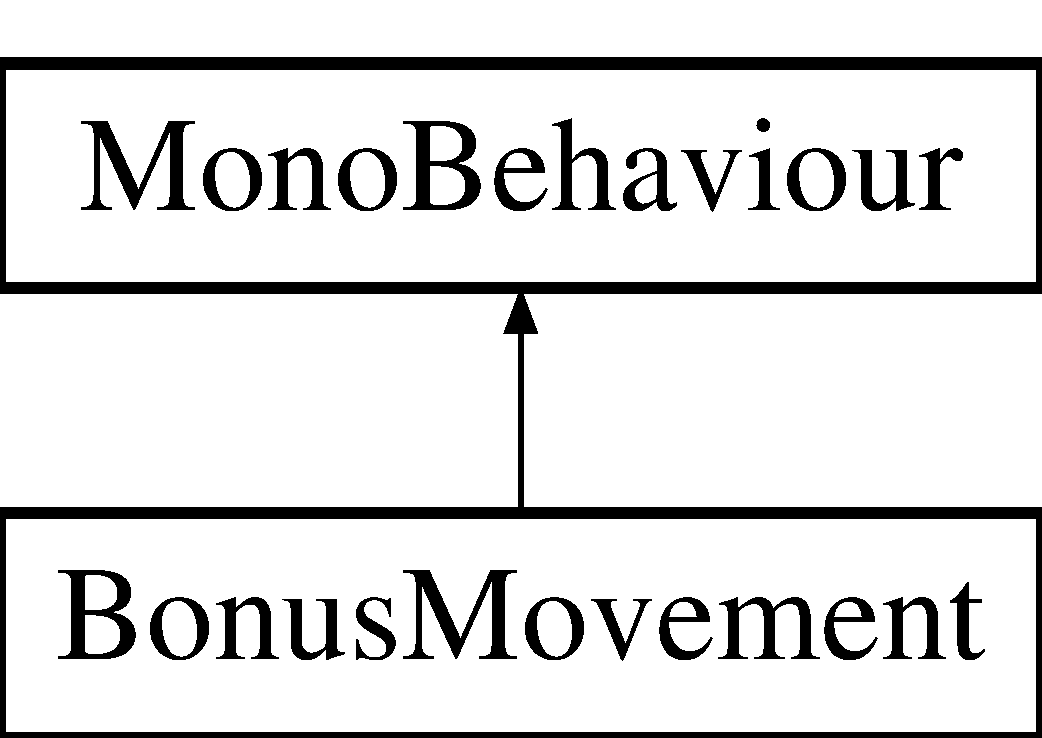
\includegraphics[height=2.000000cm]{class_bonus_movement}
\end{center}
\end{figure}
\subsection*{Public Attributes}
\begin{DoxyCompactItemize}
\item 
float \mbox{\hyperlink{class_bonus_movement_af663a81c63835c143bc17cb1f86e8e46}{speed}}
\begin{DoxyCompactList}\small\item\em Speed of bonus movement. \end{DoxyCompactList}\end{DoxyCompactItemize}


\subsection{Detailed Description}
Class responsible for movement of bonus (side, speed). 



\subsection{Member Data Documentation}
\mbox{\Hypertarget{class_bonus_movement_af663a81c63835c143bc17cb1f86e8e46}\label{class_bonus_movement_af663a81c63835c143bc17cb1f86e8e46}} 
\index{Bonus\+Movement@{Bonus\+Movement}!speed@{speed}}
\index{speed@{speed}!Bonus\+Movement@{Bonus\+Movement}}
\subsubsection{\texorpdfstring{speed}{speed}}
{\footnotesize\ttfamily float Bonus\+Movement.\+speed}



Speed of bonus movement. 



The documentation for this class was generated from the following file\+:\begin{DoxyCompactItemize}
\item 
background tasks/Bonus\+Movement.\+cs\end{DoxyCompactItemize}

\hypertarget{class_bullet_movement}{}\section{Bullet\+Movement Class Reference}
\label{class_bullet_movement}\index{Bullet\+Movement@{Bullet\+Movement}}


The movement of the bullet, including parts where it rotates around a planet.  


Inheritance diagram for Bullet\+Movement\+:\begin{figure}[H]
\begin{center}
\leavevmode
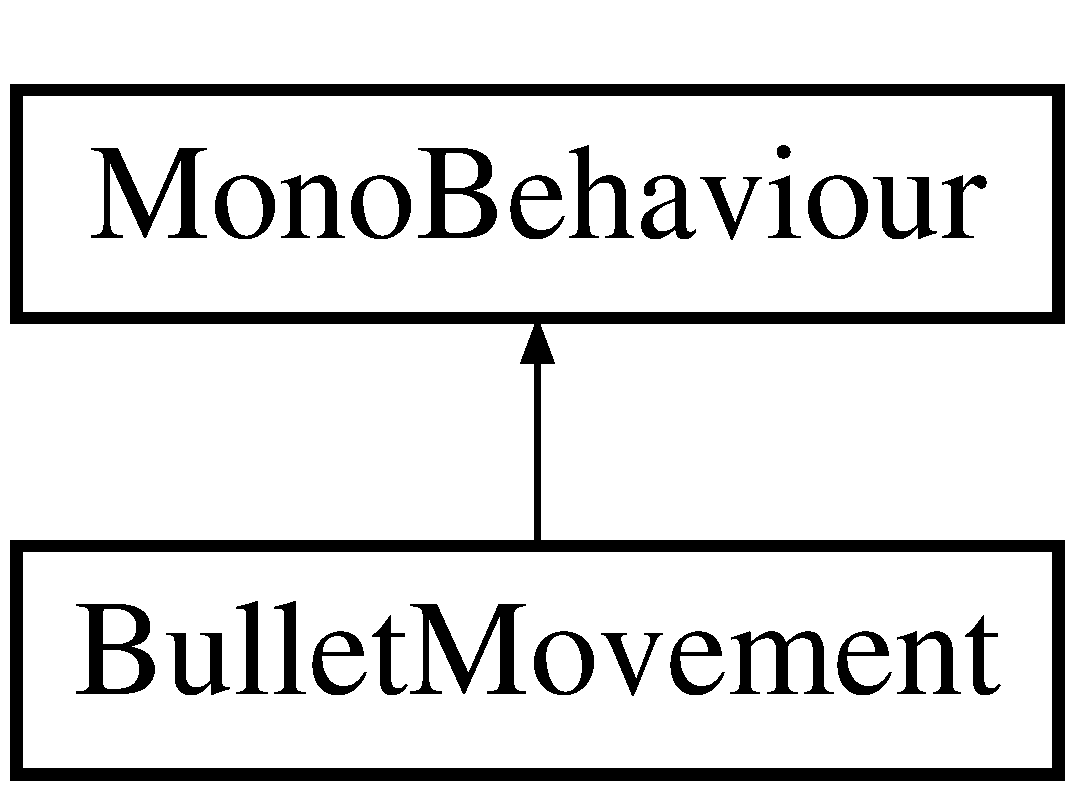
\includegraphics[height=2.000000cm]{class_bullet_movement}
\end{center}
\end{figure}
\subsection*{Public Attributes}
\begin{DoxyCompactItemize}
\item 
int \mbox{\hyperlink{class_bullet_movement_a87f4f6ec7b16819ee058cfc9121660e0}{x\+Direction\+Coeffcient}}
\begin{DoxyCompactList}\small\item\em The x direction coeffcient. \end{DoxyCompactList}\item 
float \mbox{\hyperlink{class_bullet_movement_aeb1ed7a8c4bd668bb3039562e46fa63b}{speed}} = 500
\begin{DoxyCompactList}\small\item\em The speed. \end{DoxyCompactList}\end{DoxyCompactItemize}
\subsection*{Private Member Functions}
\begin{DoxyCompactItemize}
\item 
void \mbox{\hyperlink{class_bullet_movement_aedea440e001bde34585c344da0557b6e}{Start}} ()
\begin{DoxyCompactList}\small\item\em Initializes bounds of view and the movement vector. \end{DoxyCompactList}\item 
void \mbox{\hyperlink{class_bullet_movement_a95545abaf23c8a2120076127df594db3}{Update}} ()
\begin{DoxyCompactList}\small\item\em Update this bullet. The rotate and if it is out of window destroy object \end{DoxyCompactList}\item 
bool \mbox{\hyperlink{class_bullet_movement_ab6f9452d6eefa893c167e52c285d7ce9}{is\+In\+Window}} ()
\begin{DoxyCompactList}\small\item\em check if the bullet is in the window \end{DoxyCompactList}\item 
void \mbox{\hyperlink{class_bullet_movement_a331fc1849938f5faf8aec9999f288d4c}{On\+Collision\+Stay}} (Collision col)
\begin{DoxyCompactList}\small\item\em the rotating movement on collision with planet \end{DoxyCompactList}\end{DoxyCompactItemize}
\subsection*{Private Attributes}
\begin{DoxyCompactItemize}
\item 
Vector3 \mbox{\hyperlink{class_bullet_movement_a5419583958b87067b7c8b89b2b1c6b09}{shoot\+Current}}
\begin{DoxyCompactList}\small\item\em Vector of bullet movement. \end{DoxyCompactList}\item 
float \mbox{\hyperlink{class_bullet_movement_a8e039f4911be004e48a1f2620380c15c}{rotation\+Speed}} = 100.\+0f
\begin{DoxyCompactList}\small\item\em The speed of rotation around planet in degrees per second. \end{DoxyCompactList}\item 
Game\+Object \mbox{\hyperlink{class_bullet_movement_a93263de8f413e1abcbf57f3b30b37e50}{planet}}
\begin{DoxyCompactList}\small\item\em Planet the bullet is colliding with. \end{DoxyCompactList}\item 
const string \mbox{\hyperlink{class_bullet_movement_a8a39e066bf0f84fd7ec143eea687ab12}{planet\+Tag}} = \char`\"{}Planet\char`\"{}
\begin{DoxyCompactList}\small\item\em Planet the bullet is colliding with. \end{DoxyCompactList}\end{DoxyCompactItemize}


\subsection{Detailed Description}
The movement of the bullet, including parts where it rotates around a planet. 



\subsection{Member Function Documentation}
\mbox{\Hypertarget{class_bullet_movement_ab6f9452d6eefa893c167e52c285d7ce9}\label{class_bullet_movement_ab6f9452d6eefa893c167e52c285d7ce9}} 
\index{Bullet\+Movement@{Bullet\+Movement}!is\+In\+Window@{is\+In\+Window}}
\index{is\+In\+Window@{is\+In\+Window}!Bullet\+Movement@{Bullet\+Movement}}
\subsubsection{\texorpdfstring{is\+In\+Window()}{isInWindow()}}
{\footnotesize\ttfamily bool Bullet\+Movement.\+is\+In\+Window (\begin{DoxyParamCaption}{ }\end{DoxyParamCaption})\hspace{0.3cm}{\ttfamily [private]}}



check if the bullet is in the window 

\begin{DoxyReturn}{Returns}
{\ttfamily true}, if in window was ised, {\ttfamily false} otherwise.
\end{DoxyReturn}
\mbox{\Hypertarget{class_bullet_movement_a331fc1849938f5faf8aec9999f288d4c}\label{class_bullet_movement_a331fc1849938f5faf8aec9999f288d4c}} 
\index{Bullet\+Movement@{Bullet\+Movement}!On\+Collision\+Stay@{On\+Collision\+Stay}}
\index{On\+Collision\+Stay@{On\+Collision\+Stay}!Bullet\+Movement@{Bullet\+Movement}}
\subsubsection{\texorpdfstring{On\+Collision\+Stay()}{OnCollisionStay()}}
{\footnotesize\ttfamily void Bullet\+Movement.\+On\+Collision\+Stay (\begin{DoxyParamCaption}\item[{Collision}]{col }\end{DoxyParamCaption})\hspace{0.3cm}{\ttfamily [private]}}



the rotating movement on collision with planet 


\begin{DoxyParams}{Parameters}
{\em col} & Col.\\
\hline
\end{DoxyParams}
\mbox{\Hypertarget{class_bullet_movement_aedea440e001bde34585c344da0557b6e}\label{class_bullet_movement_aedea440e001bde34585c344da0557b6e}} 
\index{Bullet\+Movement@{Bullet\+Movement}!Start@{Start}}
\index{Start@{Start}!Bullet\+Movement@{Bullet\+Movement}}
\subsubsection{\texorpdfstring{Start()}{Start()}}
{\footnotesize\ttfamily void Bullet\+Movement.\+Start (\begin{DoxyParamCaption}{ }\end{DoxyParamCaption})\hspace{0.3cm}{\ttfamily [private]}}



Initializes bounds of view and the movement vector. 

\mbox{\Hypertarget{class_bullet_movement_a95545abaf23c8a2120076127df594db3}\label{class_bullet_movement_a95545abaf23c8a2120076127df594db3}} 
\index{Bullet\+Movement@{Bullet\+Movement}!Update@{Update}}
\index{Update@{Update}!Bullet\+Movement@{Bullet\+Movement}}
\subsubsection{\texorpdfstring{Update()}{Update()}}
{\footnotesize\ttfamily void Bullet\+Movement.\+Update (\begin{DoxyParamCaption}{ }\end{DoxyParamCaption})\hspace{0.3cm}{\ttfamily [private]}}



Update this bullet. The rotate and if it is out of window destroy object 



\subsection{Member Data Documentation}
\mbox{\Hypertarget{class_bullet_movement_a93263de8f413e1abcbf57f3b30b37e50}\label{class_bullet_movement_a93263de8f413e1abcbf57f3b30b37e50}} 
\index{Bullet\+Movement@{Bullet\+Movement}!planet@{planet}}
\index{planet@{planet}!Bullet\+Movement@{Bullet\+Movement}}
\subsubsection{\texorpdfstring{planet}{planet}}
{\footnotesize\ttfamily Game\+Object Bullet\+Movement.\+planet\hspace{0.3cm}{\ttfamily [private]}}



Planet the bullet is colliding with. 

\mbox{\Hypertarget{class_bullet_movement_a8a39e066bf0f84fd7ec143eea687ab12}\label{class_bullet_movement_a8a39e066bf0f84fd7ec143eea687ab12}} 
\index{Bullet\+Movement@{Bullet\+Movement}!planet\+Tag@{planet\+Tag}}
\index{planet\+Tag@{planet\+Tag}!Bullet\+Movement@{Bullet\+Movement}}
\subsubsection{\texorpdfstring{planet\+Tag}{planetTag}}
{\footnotesize\ttfamily const string Bullet\+Movement.\+planet\+Tag = \char`\"{}Planet\char`\"{}\hspace{0.3cm}{\ttfamily [private]}}



Planet the bullet is colliding with. 

\mbox{\Hypertarget{class_bullet_movement_a8e039f4911be004e48a1f2620380c15c}\label{class_bullet_movement_a8e039f4911be004e48a1f2620380c15c}} 
\index{Bullet\+Movement@{Bullet\+Movement}!rotation\+Speed@{rotation\+Speed}}
\index{rotation\+Speed@{rotation\+Speed}!Bullet\+Movement@{Bullet\+Movement}}
\subsubsection{\texorpdfstring{rotation\+Speed}{rotationSpeed}}
{\footnotesize\ttfamily float Bullet\+Movement.\+rotation\+Speed = 100.\+0f\hspace{0.3cm}{\ttfamily [private]}}



The speed of rotation around planet in degrees per second. 

\mbox{\Hypertarget{class_bullet_movement_a5419583958b87067b7c8b89b2b1c6b09}\label{class_bullet_movement_a5419583958b87067b7c8b89b2b1c6b09}} 
\index{Bullet\+Movement@{Bullet\+Movement}!shoot\+Current@{shoot\+Current}}
\index{shoot\+Current@{shoot\+Current}!Bullet\+Movement@{Bullet\+Movement}}
\subsubsection{\texorpdfstring{shoot\+Current}{shootCurrent}}
{\footnotesize\ttfamily Vector3 Bullet\+Movement.\+shoot\+Current\hspace{0.3cm}{\ttfamily [private]}}



Vector of bullet movement. 

\mbox{\Hypertarget{class_bullet_movement_aeb1ed7a8c4bd668bb3039562e46fa63b}\label{class_bullet_movement_aeb1ed7a8c4bd668bb3039562e46fa63b}} 
\index{Bullet\+Movement@{Bullet\+Movement}!speed@{speed}}
\index{speed@{speed}!Bullet\+Movement@{Bullet\+Movement}}
\subsubsection{\texorpdfstring{speed}{speed}}
{\footnotesize\ttfamily float Bullet\+Movement.\+speed = 500}



The speed. 

\mbox{\Hypertarget{class_bullet_movement_a87f4f6ec7b16819ee058cfc9121660e0}\label{class_bullet_movement_a87f4f6ec7b16819ee058cfc9121660e0}} 
\index{Bullet\+Movement@{Bullet\+Movement}!x\+Direction\+Coeffcient@{x\+Direction\+Coeffcient}}
\index{x\+Direction\+Coeffcient@{x\+Direction\+Coeffcient}!Bullet\+Movement@{Bullet\+Movement}}
\subsubsection{\texorpdfstring{x\+Direction\+Coeffcient}{xDirectionCoeffcient}}
{\footnotesize\ttfamily int Bullet\+Movement.\+x\+Direction\+Coeffcient}



The x direction coeffcient. 



The documentation for this class was generated from the following file\+:\begin{DoxyCompactItemize}
\item 
Bullet\+Movement.\+cs\end{DoxyCompactItemize}

\hypertarget{class_calculate_screen_bounds}{}\section{Calculate\+Screen\+Bounds Class Reference}
\label{class_calculate_screen_bounds}\index{Calculate\+Screen\+Bounds@{Calculate\+Screen\+Bounds}}


Class responsible for calculating screen bounds, depending on resolution etc.  


Inheritance diagram for Calculate\+Screen\+Bounds\+:\begin{figure}[H]
\begin{center}
\leavevmode
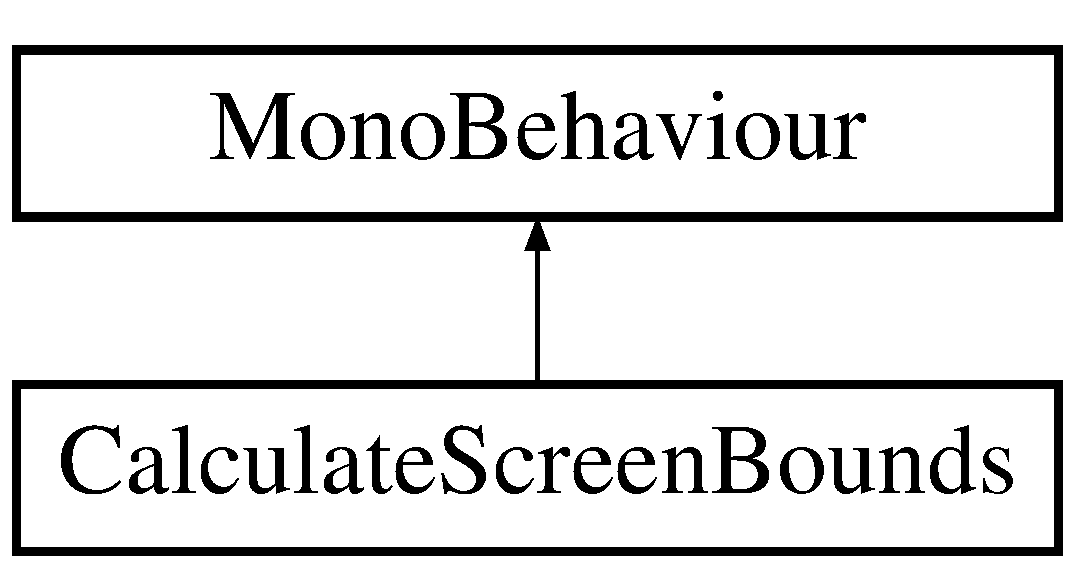
\includegraphics[height=2.000000cm]{class_calculate_screen_bounds}
\end{center}
\end{figure}
\subsection*{Static Public Member Functions}
\begin{DoxyCompactItemize}
\item 
static void \mbox{\hyperlink{class_calculate_screen_bounds_a158fa098e4529b299f223bb0e241ccc8}{calculate}} ()
\begin{DoxyCompactList}\small\item\em Method to calculate disances to vertical and horizontal bounds of view, depending on screen resolution. \end{DoxyCompactList}\end{DoxyCompactItemize}
\subsection*{Static Public Attributes}
\begin{DoxyCompactItemize}
\item 
static float \mbox{\hyperlink{class_calculate_screen_bounds_ae23c6986f2ecddbfd38c00c7bfc6855f}{distance\+To\+Vertical\+Bound\+Of\+View}}
\begin{DoxyCompactList}\small\item\em Distance to vertical bound of view from the centre of camera direct. \end{DoxyCompactList}\item 
static float \mbox{\hyperlink{class_calculate_screen_bounds_a439f514c9f28391b0b90ad9b8050e35a}{distance\+To\+Horizontal\+Bound\+Of\+View}}
\begin{DoxyCompactList}\small\item\em Distance to horizontal bound of view from the centre of camera direct. \end{DoxyCompactList}\end{DoxyCompactItemize}


\subsection{Detailed Description}
Class responsible for calculating screen bounds, depending on resolution etc. 



\subsection{Member Function Documentation}
\mbox{\Hypertarget{class_calculate_screen_bounds_a158fa098e4529b299f223bb0e241ccc8}\label{class_calculate_screen_bounds_a158fa098e4529b299f223bb0e241ccc8}} 
\index{Calculate\+Screen\+Bounds@{Calculate\+Screen\+Bounds}!calculate@{calculate}}
\index{calculate@{calculate}!Calculate\+Screen\+Bounds@{Calculate\+Screen\+Bounds}}
\subsubsection{\texorpdfstring{calculate()}{calculate()}}
{\footnotesize\ttfamily static void Calculate\+Screen\+Bounds.\+calculate (\begin{DoxyParamCaption}{ }\end{DoxyParamCaption})\hspace{0.3cm}{\ttfamily [static]}}



Method to calculate disances to vertical and horizontal bounds of view, depending on screen resolution. 



\subsection{Member Data Documentation}
\mbox{\Hypertarget{class_calculate_screen_bounds_a439f514c9f28391b0b90ad9b8050e35a}\label{class_calculate_screen_bounds_a439f514c9f28391b0b90ad9b8050e35a}} 
\index{Calculate\+Screen\+Bounds@{Calculate\+Screen\+Bounds}!distance\+To\+Horizontal\+Bound\+Of\+View@{distance\+To\+Horizontal\+Bound\+Of\+View}}
\index{distance\+To\+Horizontal\+Bound\+Of\+View@{distance\+To\+Horizontal\+Bound\+Of\+View}!Calculate\+Screen\+Bounds@{Calculate\+Screen\+Bounds}}
\subsubsection{\texorpdfstring{distance\+To\+Horizontal\+Bound\+Of\+View}{distanceToHorizontalBoundOfView}}
{\footnotesize\ttfamily float Calculate\+Screen\+Bounds.\+distance\+To\+Horizontal\+Bound\+Of\+View\hspace{0.3cm}{\ttfamily [static]}}



Distance to horizontal bound of view from the centre of camera direct. 

\mbox{\Hypertarget{class_calculate_screen_bounds_ae23c6986f2ecddbfd38c00c7bfc6855f}\label{class_calculate_screen_bounds_ae23c6986f2ecddbfd38c00c7bfc6855f}} 
\index{Calculate\+Screen\+Bounds@{Calculate\+Screen\+Bounds}!distance\+To\+Vertical\+Bound\+Of\+View@{distance\+To\+Vertical\+Bound\+Of\+View}}
\index{distance\+To\+Vertical\+Bound\+Of\+View@{distance\+To\+Vertical\+Bound\+Of\+View}!Calculate\+Screen\+Bounds@{Calculate\+Screen\+Bounds}}
\subsubsection{\texorpdfstring{distance\+To\+Vertical\+Bound\+Of\+View}{distanceToVerticalBoundOfView}}
{\footnotesize\ttfamily float Calculate\+Screen\+Bounds.\+distance\+To\+Vertical\+Bound\+Of\+View\hspace{0.3cm}{\ttfamily [static]}}



Distance to vertical bound of view from the centre of camera direct. 



The documentation for this class was generated from the following file\+:\begin{DoxyCompactItemize}
\item 
Calculate\+Screen\+Bounds.\+cs\end{DoxyCompactItemize}

\hypertarget{class_change_scene_button}{}\section{Change\+Scene\+Button Class Reference}
\label{class_change_scene_button}\index{Change\+Scene\+Button@{Change\+Scene\+Button}}


Class responsible for changing the scenes.  


Inheritance diagram for Change\+Scene\+Button\+:\begin{figure}[H]
\begin{center}
\leavevmode
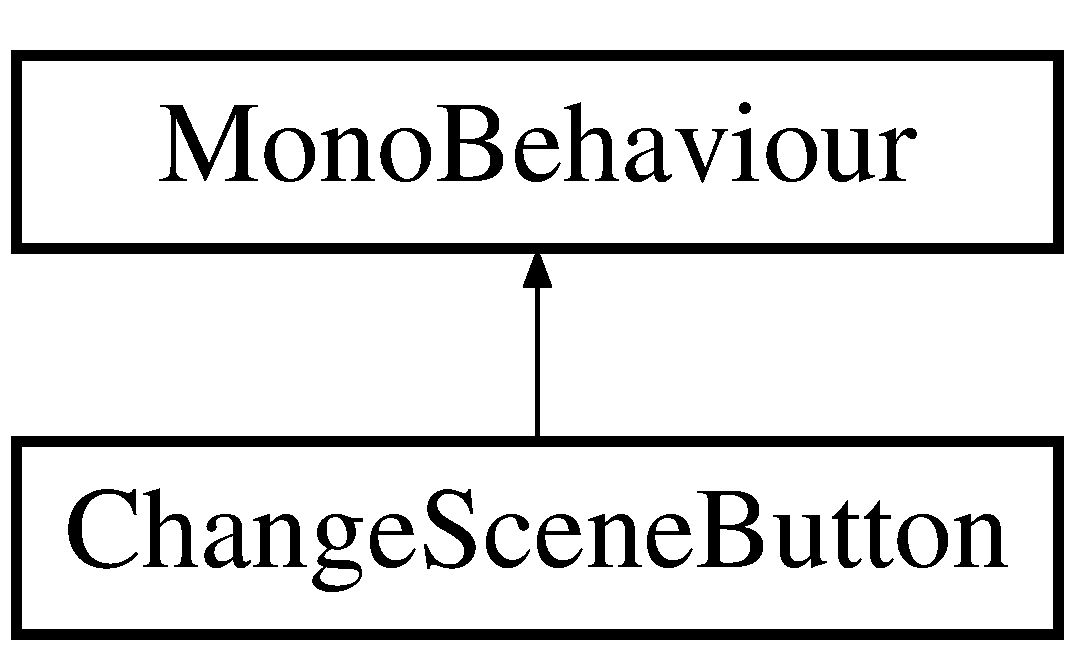
\includegraphics[height=2.000000cm]{class_change_scene_button}
\end{center}
\end{figure}
\subsection*{Public Member Functions}
\begin{DoxyCompactItemize}
\item 
void \mbox{\hyperlink{class_change_scene_button_a68b0f6974bd17f340643158594100af5}{Start\+Level}} (int level)
\begin{DoxyCompactList}\small\item\em Starts showing another scene. \end{DoxyCompactList}\end{DoxyCompactItemize}


\subsection{Detailed Description}
Class responsible for changing the scenes. 



\subsection{Member Function Documentation}
\mbox{\Hypertarget{class_change_scene_button_a68b0f6974bd17f340643158594100af5}\label{class_change_scene_button_a68b0f6974bd17f340643158594100af5}} 
\index{Change\+Scene\+Button@{Change\+Scene\+Button}!Start\+Level@{Start\+Level}}
\index{Start\+Level@{Start\+Level}!Change\+Scene\+Button@{Change\+Scene\+Button}}
\subsubsection{\texorpdfstring{Start\+Level()}{StartLevel()}}
{\footnotesize\ttfamily void Change\+Scene\+Button.\+Start\+Level (\begin{DoxyParamCaption}\item[{int}]{level }\end{DoxyParamCaption})}



Starts showing another scene. 


\begin{DoxyParams}{Parameters}
{\em level} & Scene to play.\\
\hline
\end{DoxyParams}


The documentation for this class was generated from the following file\+:\begin{DoxyCompactItemize}
\item 
menus/Change\+Scene\+Button.\+cs\end{DoxyCompactItemize}

\hypertarget{class_click_buttons}{}\section{Click\+Buttons Class Reference}
\label{class_click_buttons}\index{Click\+Buttons@{Click\+Buttons}}


Clas responsible for reacting to clicking buttons.  


Inheritance diagram for Click\+Buttons\+:\begin{figure}[H]
\begin{center}
\leavevmode
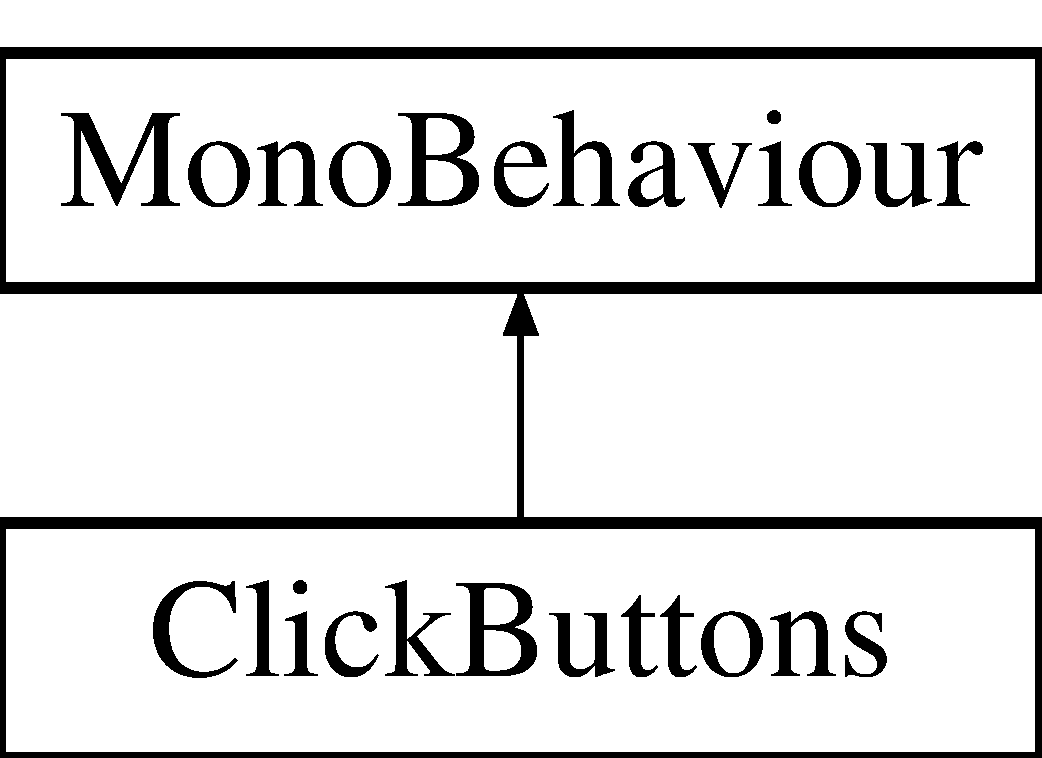
\includegraphics[height=2.000000cm]{class_click_buttons}
\end{center}
\end{figure}


\subsection{Detailed Description}
Clas responsible for reacting to clicking buttons. 



The documentation for this class was generated from the following file\+:\begin{DoxyCompactItemize}
\item 
background tasks/Click\+Buttons.\+cs\end{DoxyCompactItemize}

\hypertarget{class_collision_bullet}{}\section{Collision\+Bullet Class Reference}
\label{class_collision_bullet}\index{Collision\+Bullet@{Collision\+Bullet}}


Collision player with bullet manager  


Inheritance diagram for Collision\+Bullet\+:\begin{figure}[H]
\begin{center}
\leavevmode
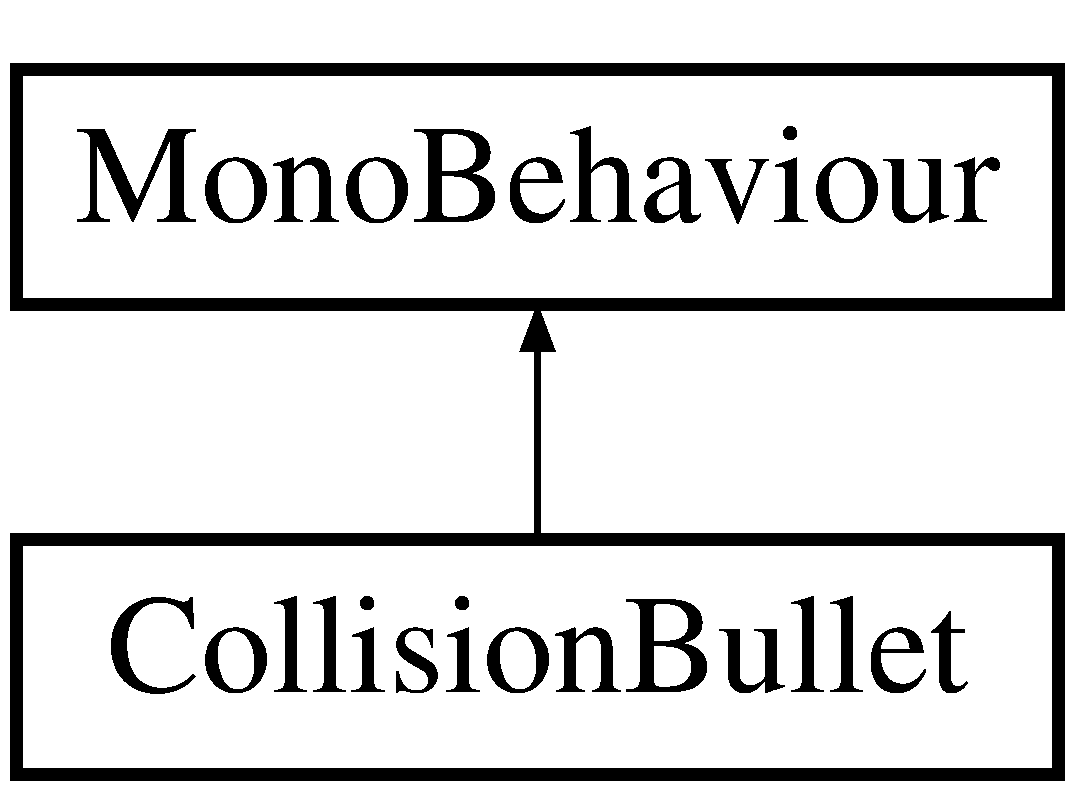
\includegraphics[height=2.000000cm]{class_collision_bullet}
\end{center}
\end{figure}
\subsection*{Public Attributes}
\begin{DoxyCompactItemize}
\item 
string \mbox{\hyperlink{class_collision_bullet_a98c6bc7c9224385999fe1226cf3c1aee}{Bullet\+Tag}}
\begin{DoxyCompactList}\small\item\em The bullet tag. \end{DoxyCompactList}\end{DoxyCompactItemize}
\subsection*{Private Member Functions}
\begin{DoxyCompactItemize}
\item 
void \mbox{\hyperlink{class_collision_bullet_a3267b5fa5550db284da7c7cbf25498f1}{On\+Collision\+Enter}} (Collision col)
\begin{DoxyCompactList}\small\item\em On collision with bullet decrement number of player\textquotesingle{}s lives \end{DoxyCompactList}\end{DoxyCompactItemize}


\subsection{Detailed Description}
Collision player with bullet manager 



\subsection{Member Function Documentation}
\mbox{\Hypertarget{class_collision_bullet_a3267b5fa5550db284da7c7cbf25498f1}\label{class_collision_bullet_a3267b5fa5550db284da7c7cbf25498f1}} 
\index{Collision\+Bullet@{Collision\+Bullet}!On\+Collision\+Enter@{On\+Collision\+Enter}}
\index{On\+Collision\+Enter@{On\+Collision\+Enter}!Collision\+Bullet@{Collision\+Bullet}}
\subsubsection{\texorpdfstring{On\+Collision\+Enter()}{OnCollisionEnter()}}
{\footnotesize\ttfamily void Collision\+Bullet.\+On\+Collision\+Enter (\begin{DoxyParamCaption}\item[{Collision}]{col }\end{DoxyParamCaption})\hspace{0.3cm}{\ttfamily [private]}}



On collision with bullet decrement number of player\textquotesingle{}s lives 


\begin{DoxyParams}{Parameters}
{\em col} & Col.\\
\hline
\end{DoxyParams}


\subsection{Member Data Documentation}
\mbox{\Hypertarget{class_collision_bullet_a98c6bc7c9224385999fe1226cf3c1aee}\label{class_collision_bullet_a98c6bc7c9224385999fe1226cf3c1aee}} 
\index{Collision\+Bullet@{Collision\+Bullet}!Bullet\+Tag@{Bullet\+Tag}}
\index{Bullet\+Tag@{Bullet\+Tag}!Collision\+Bullet@{Collision\+Bullet}}
\subsubsection{\texorpdfstring{Bullet\+Tag}{BulletTag}}
{\footnotesize\ttfamily string Collision\+Bullet.\+Bullet\+Tag}



The bullet tag. 



The documentation for this class was generated from the following file\+:\begin{DoxyCompactItemize}
\item 
Player/\+Bullet/Collision\+Bullet.\+cs\end{DoxyCompactItemize}

\hypertarget{class_game_over}{}\section{Game\+Over Class Reference}
\label{class_game_over}\index{Game\+Over@{Game\+Over}}


Class responsible of showing \char`\"{}\+Game Over\char`\"{} canvas if one player looses.  


Inheritance diagram for Game\+Over\+:\begin{figure}[H]
\begin{center}
\leavevmode
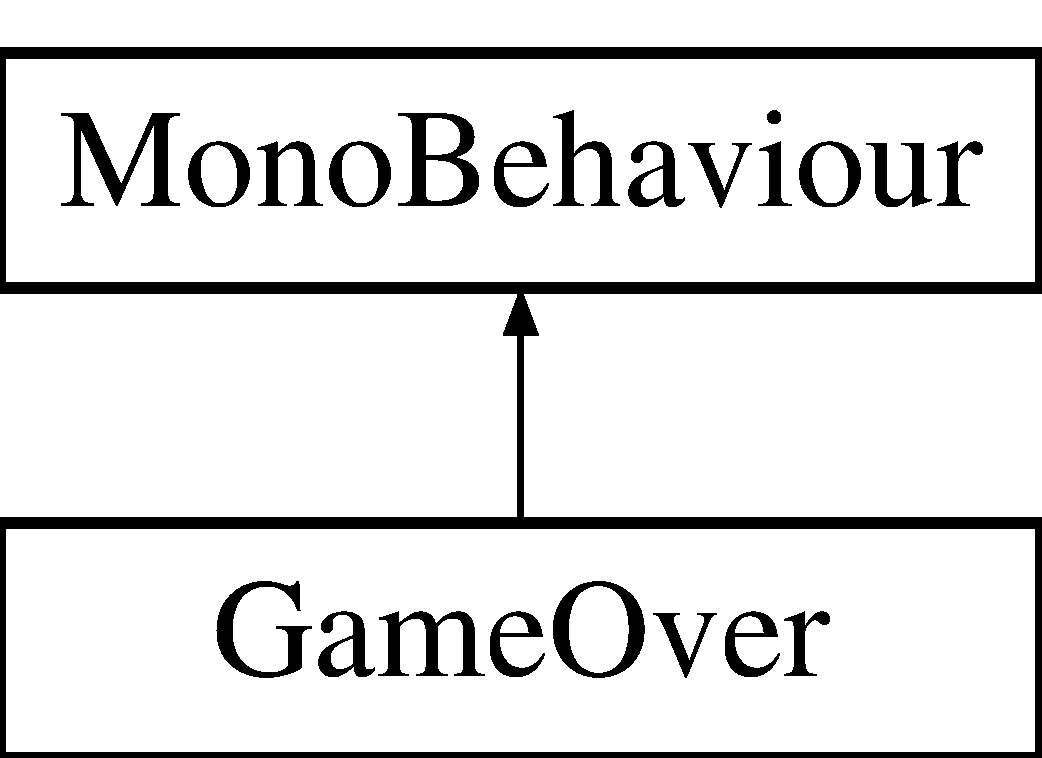
\includegraphics[height=2.000000cm]{class_game_over}
\end{center}
\end{figure}
\subsection*{Public Member Functions}
\begin{DoxyCompactItemize}
\item 
void \mbox{\hyperlink{class_game_over_a03d824dff5b997d7566f5e7bb5326609}{game\+Over}} ()
\begin{DoxyCompactList}\small\item\em Sets game over info to show on the canvas. \end{DoxyCompactList}\end{DoxyCompactItemize}
\subsection*{Public Attributes}
\begin{DoxyCompactItemize}
\item 
Text \mbox{\hyperlink{class_game_over_a05fc5c0c7a78b9a32de2bd9a9bfcac57}{text\+Who\+Won}}
\begin{DoxyCompactList}\small\item\em Text of winner\textquotesingle{}s name. \end{DoxyCompactList}\item 
Transform \mbox{\hyperlink{class_game_over_ad71e27e7f62da1f7abba74e31d89e9d5}{canvas}}
\begin{DoxyCompactList}\small\item\em Canvas with game over info. \end{DoxyCompactList}\end{DoxyCompactItemize}
\subsection*{Private Member Functions}
\begin{DoxyCompactItemize}
\item 
void \mbox{\hyperlink{class_game_over_a568be230765aad02fc07c3ff2d655e41}{Start}} ()
\begin{DoxyCompactList}\small\item\em At the beginning of the game, \char`\"{}\+Game Over\char`\"{} canvas should not be shown. \end{DoxyCompactList}\item 
void \mbox{\hyperlink{class_game_over_ab9acefb17781e10acace7ea576d48d63}{Update}} ()
\begin{DoxyCompactList}\small\item\em If this class is activated, it should show \char`\"{}\+Game Over\char`\"{} canvas. \end{DoxyCompactList}\item 
void \mbox{\hyperlink{class_game_over_a8dc8ae299906de6009ed0e7ae65b7ca9}{deactive\+Scene}} ()
\begin{DoxyCompactList}\small\item\em Deactivates playing scene and shows \char`\"{}\+Game Over\char`\"{} canvas. \end{DoxyCompactList}\end{DoxyCompactItemize}


\subsection{Detailed Description}
Class responsible of showing \char`\"{}\+Game Over\char`\"{} canvas if one player looses. 



\subsection{Member Function Documentation}
\mbox{\Hypertarget{class_game_over_a8dc8ae299906de6009ed0e7ae65b7ca9}\label{class_game_over_a8dc8ae299906de6009ed0e7ae65b7ca9}} 
\index{Game\+Over@{Game\+Over}!deactive\+Scene@{deactive\+Scene}}
\index{deactive\+Scene@{deactive\+Scene}!Game\+Over@{Game\+Over}}
\subsubsection{\texorpdfstring{deactive\+Scene()}{deactiveScene()}}
{\footnotesize\ttfamily void Game\+Over.\+deactive\+Scene (\begin{DoxyParamCaption}{ }\end{DoxyParamCaption})\hspace{0.3cm}{\ttfamily [private]}}



Deactivates playing scene and shows \char`\"{}\+Game Over\char`\"{} canvas. 

\mbox{\Hypertarget{class_game_over_a03d824dff5b997d7566f5e7bb5326609}\label{class_game_over_a03d824dff5b997d7566f5e7bb5326609}} 
\index{Game\+Over@{Game\+Over}!game\+Over@{game\+Over}}
\index{game\+Over@{game\+Over}!Game\+Over@{Game\+Over}}
\subsubsection{\texorpdfstring{game\+Over()}{gameOver()}}
{\footnotesize\ttfamily void Game\+Over.\+game\+Over (\begin{DoxyParamCaption}{ }\end{DoxyParamCaption})}



Sets game over info to show on the canvas. 

\mbox{\Hypertarget{class_game_over_a568be230765aad02fc07c3ff2d655e41}\label{class_game_over_a568be230765aad02fc07c3ff2d655e41}} 
\index{Game\+Over@{Game\+Over}!Start@{Start}}
\index{Start@{Start}!Game\+Over@{Game\+Over}}
\subsubsection{\texorpdfstring{Start()}{Start()}}
{\footnotesize\ttfamily void Game\+Over.\+Start (\begin{DoxyParamCaption}{ }\end{DoxyParamCaption})\hspace{0.3cm}{\ttfamily [private]}}



At the beginning of the game, \char`\"{}\+Game Over\char`\"{} canvas should not be shown. 

\mbox{\Hypertarget{class_game_over_ab9acefb17781e10acace7ea576d48d63}\label{class_game_over_ab9acefb17781e10acace7ea576d48d63}} 
\index{Game\+Over@{Game\+Over}!Update@{Update}}
\index{Update@{Update}!Game\+Over@{Game\+Over}}
\subsubsection{\texorpdfstring{Update()}{Update()}}
{\footnotesize\ttfamily void Game\+Over.\+Update (\begin{DoxyParamCaption}{ }\end{DoxyParamCaption})\hspace{0.3cm}{\ttfamily [private]}}



If this class is activated, it should show \char`\"{}\+Game Over\char`\"{} canvas. 



\subsection{Member Data Documentation}
\mbox{\Hypertarget{class_game_over_ad71e27e7f62da1f7abba74e31d89e9d5}\label{class_game_over_ad71e27e7f62da1f7abba74e31d89e9d5}} 
\index{Game\+Over@{Game\+Over}!canvas@{canvas}}
\index{canvas@{canvas}!Game\+Over@{Game\+Over}}
\subsubsection{\texorpdfstring{canvas}{canvas}}
{\footnotesize\ttfamily Transform Game\+Over.\+canvas}



Canvas with game over info. 

\mbox{\Hypertarget{class_game_over_a05fc5c0c7a78b9a32de2bd9a9bfcac57}\label{class_game_over_a05fc5c0c7a78b9a32de2bd9a9bfcac57}} 
\index{Game\+Over@{Game\+Over}!text\+Who\+Won@{text\+Who\+Won}}
\index{text\+Who\+Won@{text\+Who\+Won}!Game\+Over@{Game\+Over}}
\subsubsection{\texorpdfstring{text\+Who\+Won}{textWhoWon}}
{\footnotesize\ttfamily Text Game\+Over.\+text\+Who\+Won}



Text of winner\textquotesingle{}s name. 



The documentation for this class was generated from the following file\+:\begin{DoxyCompactItemize}
\item 
menus/Game\+Over.\+cs\end{DoxyCompactItemize}

\hypertarget{class_instantiate_bullet}{}\section{Instantiate\+Bullet Class Reference}
\label{class_instantiate_bullet}\index{Instantiate\+Bullet@{Instantiate\+Bullet}}


Instantiate bullet.  


Inheritance diagram for Instantiate\+Bullet\+:\begin{figure}[H]
\begin{center}
\leavevmode
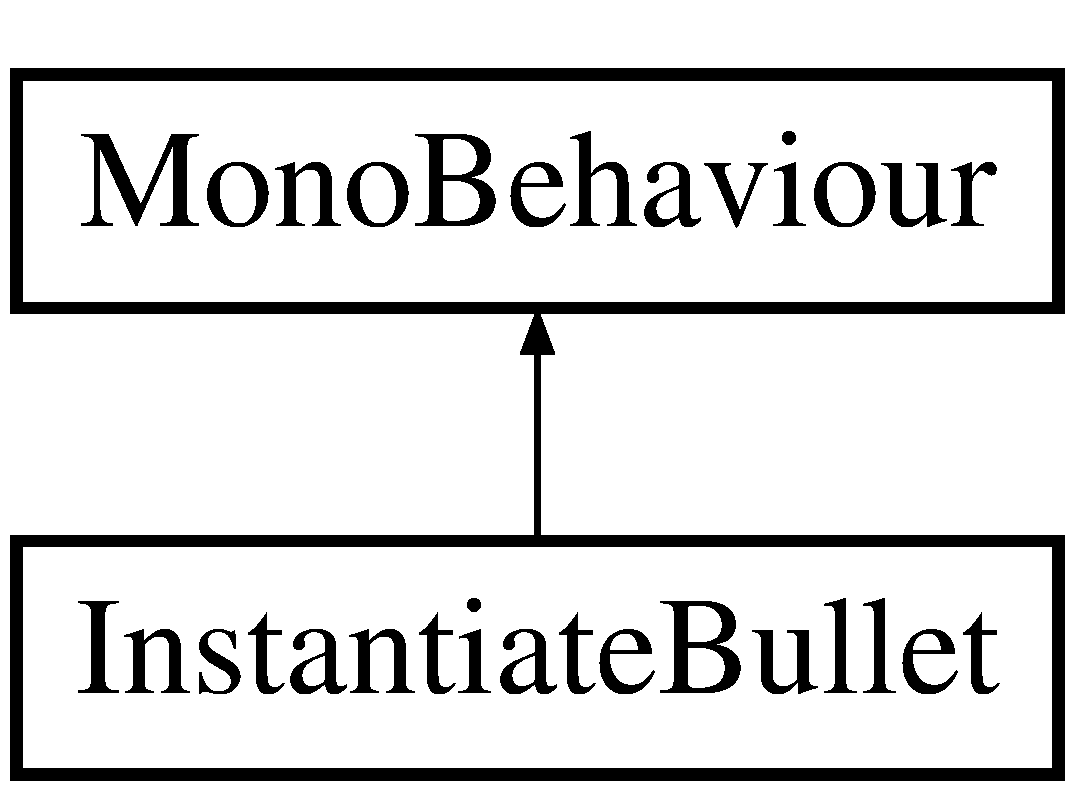
\includegraphics[height=2.000000cm]{class_instantiate_bullet}
\end{center}
\end{figure}
\subsection*{Public Attributes}
\begin{DoxyCompactItemize}
\item 
Game\+Object \mbox{\hyperlink{class_instantiate_bullet_a5f592b6ea8184022a425de7fb34cd1c8}{bullet}}
\begin{DoxyCompactList}\small\item\em The bullet. \end{DoxyCompactList}\item 
string \mbox{\hyperlink{class_instantiate_bullet_a3eebc503e154a693e632bf480b2209c4}{Bullet\+Tag}}
\begin{DoxyCompactList}\small\item\em The bullet tag. \end{DoxyCompactList}\end{DoxyCompactItemize}
\subsection*{Private Member Functions}
\begin{DoxyCompactItemize}
\item 
void \mbox{\hyperlink{class_instantiate_bullet_aedc5efe186e3d0ad9639c58be67088ac}{Start}} ()
\begin{DoxyCompactList}\small\item\em set the player\textquotesingle{}s default rate of fire \end{DoxyCompactList}\item 
void \mbox{\hyperlink{class_instantiate_bullet_a0a6f4639d59779ad8d5ef7de4ef5234c}{Update}} ()
\begin{DoxyCompactList}\small\item\em update if the player can shot \end{DoxyCompactList}\end{DoxyCompactItemize}
\subsection*{Private Attributes}
\begin{DoxyCompactItemize}
\item 
float \mbox{\hyperlink{class_instantiate_bullet_a6616ff47defe7c35d2ce6bea1b9e871a}{current\+Rate}}
\begin{DoxyCompactList}\small\item\em Curret bullet rate. \end{DoxyCompactList}\end{DoxyCompactItemize}


\subsection{Detailed Description}
Instantiate bullet. 



\subsection{Member Function Documentation}
\mbox{\Hypertarget{class_instantiate_bullet_aedc5efe186e3d0ad9639c58be67088ac}\label{class_instantiate_bullet_aedc5efe186e3d0ad9639c58be67088ac}} 
\index{Instantiate\+Bullet@{Instantiate\+Bullet}!Start@{Start}}
\index{Start@{Start}!Instantiate\+Bullet@{Instantiate\+Bullet}}
\subsubsection{\texorpdfstring{Start()}{Start()}}
{\footnotesize\ttfamily void Instantiate\+Bullet.\+Start (\begin{DoxyParamCaption}{ }\end{DoxyParamCaption})\hspace{0.3cm}{\ttfamily [private]}}



set the player\textquotesingle{}s default rate of fire 

\mbox{\Hypertarget{class_instantiate_bullet_a0a6f4639d59779ad8d5ef7de4ef5234c}\label{class_instantiate_bullet_a0a6f4639d59779ad8d5ef7de4ef5234c}} 
\index{Instantiate\+Bullet@{Instantiate\+Bullet}!Update@{Update}}
\index{Update@{Update}!Instantiate\+Bullet@{Instantiate\+Bullet}}
\subsubsection{\texorpdfstring{Update()}{Update()}}
{\footnotesize\ttfamily void Instantiate\+Bullet.\+Update (\begin{DoxyParamCaption}{ }\end{DoxyParamCaption})\hspace{0.3cm}{\ttfamily [private]}}



update if the player can shot 



\subsection{Member Data Documentation}
\mbox{\Hypertarget{class_instantiate_bullet_a5f592b6ea8184022a425de7fb34cd1c8}\label{class_instantiate_bullet_a5f592b6ea8184022a425de7fb34cd1c8}} 
\index{Instantiate\+Bullet@{Instantiate\+Bullet}!bullet@{bullet}}
\index{bullet@{bullet}!Instantiate\+Bullet@{Instantiate\+Bullet}}
\subsubsection{\texorpdfstring{bullet}{bullet}}
{\footnotesize\ttfamily Game\+Object Instantiate\+Bullet.\+bullet}



The bullet. 

\mbox{\Hypertarget{class_instantiate_bullet_a3eebc503e154a693e632bf480b2209c4}\label{class_instantiate_bullet_a3eebc503e154a693e632bf480b2209c4}} 
\index{Instantiate\+Bullet@{Instantiate\+Bullet}!Bullet\+Tag@{Bullet\+Tag}}
\index{Bullet\+Tag@{Bullet\+Tag}!Instantiate\+Bullet@{Instantiate\+Bullet}}
\subsubsection{\texorpdfstring{Bullet\+Tag}{BulletTag}}
{\footnotesize\ttfamily string Instantiate\+Bullet.\+Bullet\+Tag}



The bullet tag. 

\mbox{\Hypertarget{class_instantiate_bullet_a6616ff47defe7c35d2ce6bea1b9e871a}\label{class_instantiate_bullet_a6616ff47defe7c35d2ce6bea1b9e871a}} 
\index{Instantiate\+Bullet@{Instantiate\+Bullet}!current\+Rate@{current\+Rate}}
\index{current\+Rate@{current\+Rate}!Instantiate\+Bullet@{Instantiate\+Bullet}}
\subsubsection{\texorpdfstring{current\+Rate}{currentRate}}
{\footnotesize\ttfamily float Instantiate\+Bullet.\+current\+Rate\hspace{0.3cm}{\ttfamily [private]}}



Curret bullet rate. 



The documentation for this class was generated from the following file\+:\begin{DoxyCompactItemize}
\item 
Player/\+Bullet/Instantiate\+Bullet.\+cs\end{DoxyCompactItemize}

\hypertarget{class_move}{}\section{Move Class Reference}
\label{class_move}\index{Move@{Move}}


Class responsible for player movement.  


Inheritance diagram for Move\+:\begin{figure}[H]
\begin{center}
\leavevmode
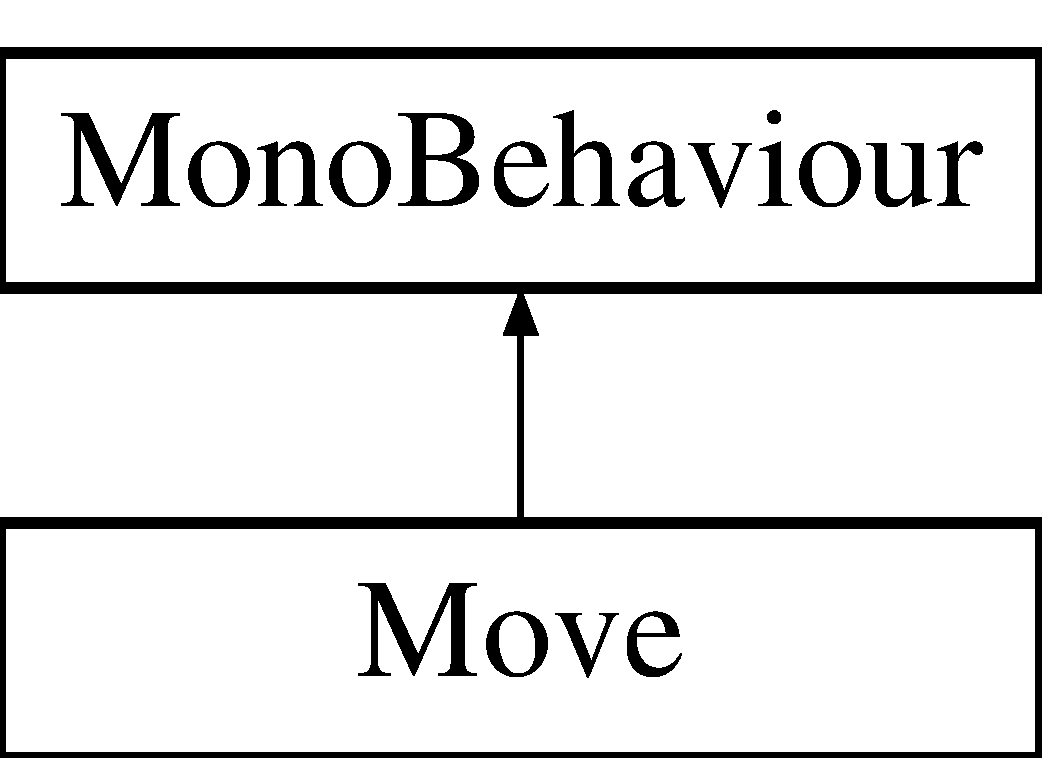
\includegraphics[height=2.000000cm]{class_move}
\end{center}
\end{figure}
\subsection*{Public Attributes}
\begin{DoxyCompactItemize}
\item 
float \mbox{\hyperlink{class_move_a248dd0919f2777f32c019ca10c342629}{move\+Vertical}}
\begin{DoxyCompactList}\small\item\em The move vertical. \end{DoxyCompactList}\item 
float \mbox{\hyperlink{class_move_a2777ede3b7fbfd425deb04fe8fd69791}{move\+Horizontal}}
\begin{DoxyCompactList}\small\item\em The move horizontal. \end{DoxyCompactList}\item 
float \mbox{\hyperlink{class_move_a564c70756027d119d684db3edfede659}{Width\+Of\+Movement}}
\begin{DoxyCompactList}\small\item\em The width of movement. \end{DoxyCompactList}\item 
Side \mbox{\hyperlink{class_move_a0cf32cb803f7b4783a49ea55c9746dba}{side}}
\begin{DoxyCompactList}\small\item\em The side. \end{DoxyCompactList}\end{DoxyCompactItemize}


\subsection{Detailed Description}
Class responsible for player movement. 



\subsection{Member Data Documentation}
\mbox{\Hypertarget{class_move_a2777ede3b7fbfd425deb04fe8fd69791}\label{class_move_a2777ede3b7fbfd425deb04fe8fd69791}} 
\index{Move@{Move}!move\+Horizontal@{move\+Horizontal}}
\index{move\+Horizontal@{move\+Horizontal}!Move@{Move}}
\subsubsection{\texorpdfstring{move\+Horizontal}{moveHorizontal}}
{\footnotesize\ttfamily float Move.\+move\+Horizontal}



The move horizontal. 

\mbox{\Hypertarget{class_move_a248dd0919f2777f32c019ca10c342629}\label{class_move_a248dd0919f2777f32c019ca10c342629}} 
\index{Move@{Move}!move\+Vertical@{move\+Vertical}}
\index{move\+Vertical@{move\+Vertical}!Move@{Move}}
\subsubsection{\texorpdfstring{move\+Vertical}{moveVertical}}
{\footnotesize\ttfamily float Move.\+move\+Vertical}



The move vertical. 

\mbox{\Hypertarget{class_move_a0cf32cb803f7b4783a49ea55c9746dba}\label{class_move_a0cf32cb803f7b4783a49ea55c9746dba}} 
\index{Move@{Move}!side@{side}}
\index{side@{side}!Move@{Move}}
\subsubsection{\texorpdfstring{side}{side}}
{\footnotesize\ttfamily Side Move.\+side}



The side. 

\mbox{\Hypertarget{class_move_a564c70756027d119d684db3edfede659}\label{class_move_a564c70756027d119d684db3edfede659}} 
\index{Move@{Move}!Width\+Of\+Movement@{Width\+Of\+Movement}}
\index{Width\+Of\+Movement@{Width\+Of\+Movement}!Move@{Move}}
\subsubsection{\texorpdfstring{Width\+Of\+Movement}{WidthOfMovement}}
{\footnotesize\ttfamily float Move.\+Width\+Of\+Movement}



The width of movement. 



The documentation for this class was generated from the following file\+:\begin{DoxyCompactItemize}
\item 
Player/Move.\+cs\end{DoxyCompactItemize}

\hypertarget{class_pause_game}{}\section{Pause\+Game Class Reference}
\label{class_pause_game}\index{Pause\+Game@{Pause\+Game}}


Class responsible of pausing the game.  


Inheritance diagram for Pause\+Game\+:\begin{figure}[H]
\begin{center}
\leavevmode
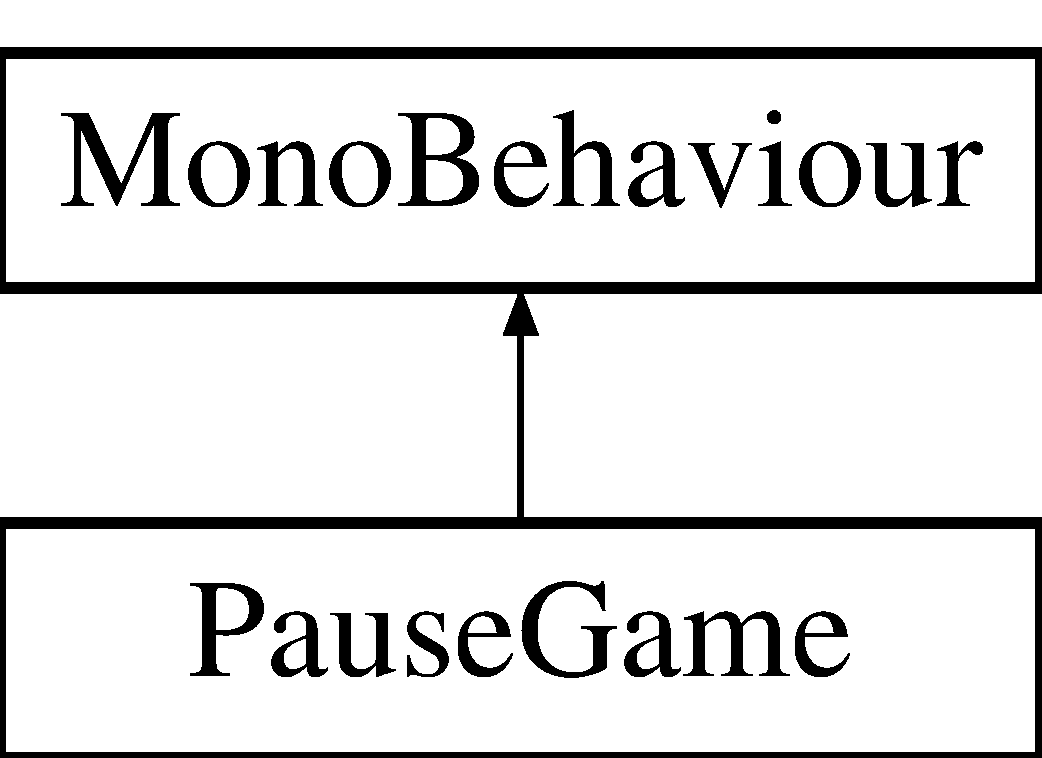
\includegraphics[height=2.000000cm]{class_pause_game}
\end{center}
\end{figure}
\subsection*{Public Member Functions}
\begin{DoxyCompactItemize}
\item 
void \mbox{\hyperlink{class_pause_game_a931478b9fc65d240b62a1cfa68607684}{Pause}} ()
\begin{DoxyCompactList}\small\item\em Pause game -\/ show \char`\"{}\+Pause Menu\char`\"{} canvas and stop all objects\textquotesingle{} movement. \end{DoxyCompactList}\item 
void \mbox{\hyperlink{class_pause_game_a70d2c89455ef1f1970d5fc7b791b7566}{Resume}} ()
\begin{DoxyCompactList}\small\item\em Unpause game -\/ go back to playing mode. \end{DoxyCompactList}\end{DoxyCompactItemize}
\subsection*{Public Attributes}
\begin{DoxyCompactItemize}
\item 
Transform \mbox{\hyperlink{class_pause_game_adf677814c2492d0887efd5ea18e6bba4}{canvas}}
\begin{DoxyCompactList}\small\item\em Canvas which is shown when pausing the game. \end{DoxyCompactList}\end{DoxyCompactItemize}
\subsection*{Private Member Functions}
\begin{DoxyCompactItemize}
\item 
void \mbox{\hyperlink{class_pause_game_ad8c1d801b6da90aee58fdd8b0b2f2b97}{Start}} ()
\begin{DoxyCompactList}\small\item\em The \char`\"{}\+Pause Menu\char`\"{} canvas must not be shown by default. \end{DoxyCompactList}\item 
void \mbox{\hyperlink{class_pause_game_ab0e714ec7b02d822c8491abba21d55fb}{Update}} ()
\begin{DoxyCompactList}\small\item\em Gam should be paused and unpaused when user clicks \char`\"{}\+Escape\char`\"{} key. \end{DoxyCompactList}\end{DoxyCompactItemize}


\subsection{Detailed Description}
Class responsible of pausing the game. 



\subsection{Member Function Documentation}
\mbox{\Hypertarget{class_pause_game_a931478b9fc65d240b62a1cfa68607684}\label{class_pause_game_a931478b9fc65d240b62a1cfa68607684}} 
\index{Pause\+Game@{Pause\+Game}!Pause@{Pause}}
\index{Pause@{Pause}!Pause\+Game@{Pause\+Game}}
\subsubsection{\texorpdfstring{Pause()}{Pause()}}
{\footnotesize\ttfamily void Pause\+Game.\+Pause (\begin{DoxyParamCaption}{ }\end{DoxyParamCaption})}



Pause game -\/ show \char`\"{}\+Pause Menu\char`\"{} canvas and stop all objects\textquotesingle{} movement. 

\mbox{\Hypertarget{class_pause_game_a70d2c89455ef1f1970d5fc7b791b7566}\label{class_pause_game_a70d2c89455ef1f1970d5fc7b791b7566}} 
\index{Pause\+Game@{Pause\+Game}!Resume@{Resume}}
\index{Resume@{Resume}!Pause\+Game@{Pause\+Game}}
\subsubsection{\texorpdfstring{Resume()}{Resume()}}
{\footnotesize\ttfamily void Pause\+Game.\+Resume (\begin{DoxyParamCaption}{ }\end{DoxyParamCaption})}



Unpause game -\/ go back to playing mode. 

\mbox{\Hypertarget{class_pause_game_ad8c1d801b6da90aee58fdd8b0b2f2b97}\label{class_pause_game_ad8c1d801b6da90aee58fdd8b0b2f2b97}} 
\index{Pause\+Game@{Pause\+Game}!Start@{Start}}
\index{Start@{Start}!Pause\+Game@{Pause\+Game}}
\subsubsection{\texorpdfstring{Start()}{Start()}}
{\footnotesize\ttfamily void Pause\+Game.\+Start (\begin{DoxyParamCaption}{ }\end{DoxyParamCaption})\hspace{0.3cm}{\ttfamily [private]}}



The \char`\"{}\+Pause Menu\char`\"{} canvas must not be shown by default. 

\mbox{\Hypertarget{class_pause_game_ab0e714ec7b02d822c8491abba21d55fb}\label{class_pause_game_ab0e714ec7b02d822c8491abba21d55fb}} 
\index{Pause\+Game@{Pause\+Game}!Update@{Update}}
\index{Update@{Update}!Pause\+Game@{Pause\+Game}}
\subsubsection{\texorpdfstring{Update()}{Update()}}
{\footnotesize\ttfamily void Pause\+Game.\+Update (\begin{DoxyParamCaption}{ }\end{DoxyParamCaption})\hspace{0.3cm}{\ttfamily [private]}}



Gam should be paused and unpaused when user clicks \char`\"{}\+Escape\char`\"{} key. 



\subsection{Member Data Documentation}
\mbox{\Hypertarget{class_pause_game_adf677814c2492d0887efd5ea18e6bba4}\label{class_pause_game_adf677814c2492d0887efd5ea18e6bba4}} 
\index{Pause\+Game@{Pause\+Game}!canvas@{canvas}}
\index{canvas@{canvas}!Pause\+Game@{Pause\+Game}}
\subsubsection{\texorpdfstring{canvas}{canvas}}
{\footnotesize\ttfamily Transform Pause\+Game.\+canvas}



Canvas which is shown when pausing the game. 



The documentation for this class was generated from the following file\+:\begin{DoxyCompactItemize}
\item 
menus/Pause\+Game.\+cs\end{DoxyCompactItemize}

\hypertarget{class_place_score_bars}{}\section{Place\+Score\+Bars Class Reference}
\label{class_place_score_bars}\index{Place\+Score\+Bars@{Place\+Score\+Bars}}


Class responsible for placing score bars.  


Inheritance diagram for Place\+Score\+Bars\+:\begin{figure}[H]
\begin{center}
\leavevmode
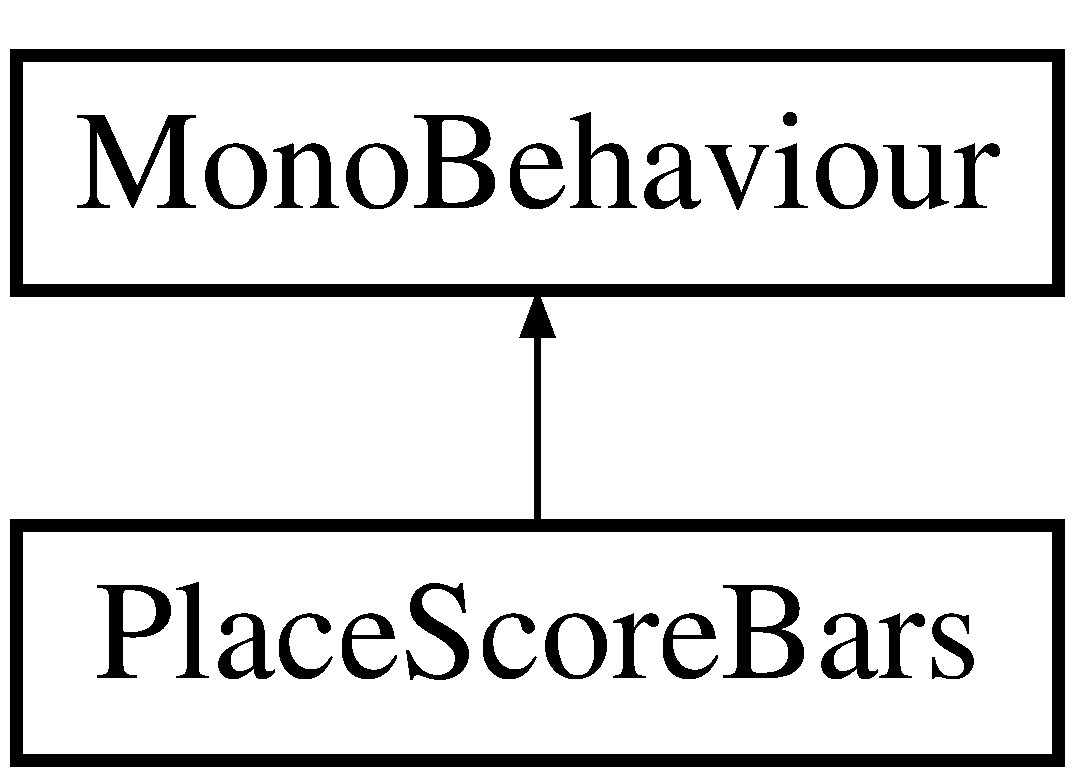
\includegraphics[height=2.000000cm]{class_place_score_bars}
\end{center}
\end{figure}
\subsection*{Public Attributes}
\begin{DoxyCompactItemize}
\item 
Image \mbox{\hyperlink{class_place_score_bars_acbdc64a22696d614a80fb2290e2e7be7}{player1\+Score}}
\begin{DoxyCompactList}\small\item\em First player\textquotesingle{}s score bar. \end{DoxyCompactList}\item 
Image \mbox{\hyperlink{class_place_score_bars_a53a2fc54c5de9160788eac17a2ff9e90}{player2\+Score}}
\begin{DoxyCompactList}\small\item\em Second player\textquotesingle{}s score bar. \end{DoxyCompactList}\end{DoxyCompactItemize}
\subsection*{Private Member Functions}
\begin{DoxyCompactItemize}
\item 
void \mbox{\hyperlink{class_place_score_bars_adf99a036ca929e8b17236267e9dc3737}{Start}} ()
\begin{DoxyCompactList}\small\item\em Counts screen bounds and places score bars in upper corners. \end{DoxyCompactList}\end{DoxyCompactItemize}


\subsection{Detailed Description}
Class responsible for placing score bars. 



\subsection{Member Function Documentation}
\mbox{\Hypertarget{class_place_score_bars_adf99a036ca929e8b17236267e9dc3737}\label{class_place_score_bars_adf99a036ca929e8b17236267e9dc3737}} 
\index{Place\+Score\+Bars@{Place\+Score\+Bars}!Start@{Start}}
\index{Start@{Start}!Place\+Score\+Bars@{Place\+Score\+Bars}}
\subsubsection{\texorpdfstring{Start()}{Start()}}
{\footnotesize\ttfamily void Place\+Score\+Bars.\+Start (\begin{DoxyParamCaption}{ }\end{DoxyParamCaption})\hspace{0.3cm}{\ttfamily [private]}}



Counts screen bounds and places score bars in upper corners. 



\subsection{Member Data Documentation}
\mbox{\Hypertarget{class_place_score_bars_acbdc64a22696d614a80fb2290e2e7be7}\label{class_place_score_bars_acbdc64a22696d614a80fb2290e2e7be7}} 
\index{Place\+Score\+Bars@{Place\+Score\+Bars}!player1\+Score@{player1\+Score}}
\index{player1\+Score@{player1\+Score}!Place\+Score\+Bars@{Place\+Score\+Bars}}
\subsubsection{\texorpdfstring{player1\+Score}{player1Score}}
{\footnotesize\ttfamily Image Place\+Score\+Bars.\+player1\+Score}



First player\textquotesingle{}s score bar. 

\mbox{\Hypertarget{class_place_score_bars_a53a2fc54c5de9160788eac17a2ff9e90}\label{class_place_score_bars_a53a2fc54c5de9160788eac17a2ff9e90}} 
\index{Place\+Score\+Bars@{Place\+Score\+Bars}!player2\+Score@{player2\+Score}}
\index{player2\+Score@{player2\+Score}!Place\+Score\+Bars@{Place\+Score\+Bars}}
\subsubsection{\texorpdfstring{player2\+Score}{player2Score}}
{\footnotesize\ttfamily Image Place\+Score\+Bars.\+player2\+Score}



Second player\textquotesingle{}s score bar. 



The documentation for this class was generated from the following file\+:\begin{DoxyCompactItemize}
\item 
background tasks/Place\+Score\+Bars.\+cs\end{DoxyCompactItemize}

\hypertarget{class_planet_lifes_controller}{}\section{Planet\+Lifes\+Controller Class Reference}
\label{class_planet_lifes_controller}\index{Planet\+Lifes\+Controller@{Planet\+Lifes\+Controller}}


Class to control planet lifes and show explosion effect after it dies.  


Inheritance diagram for Planet\+Lifes\+Controller\+:\begin{figure}[H]
\begin{center}
\leavevmode
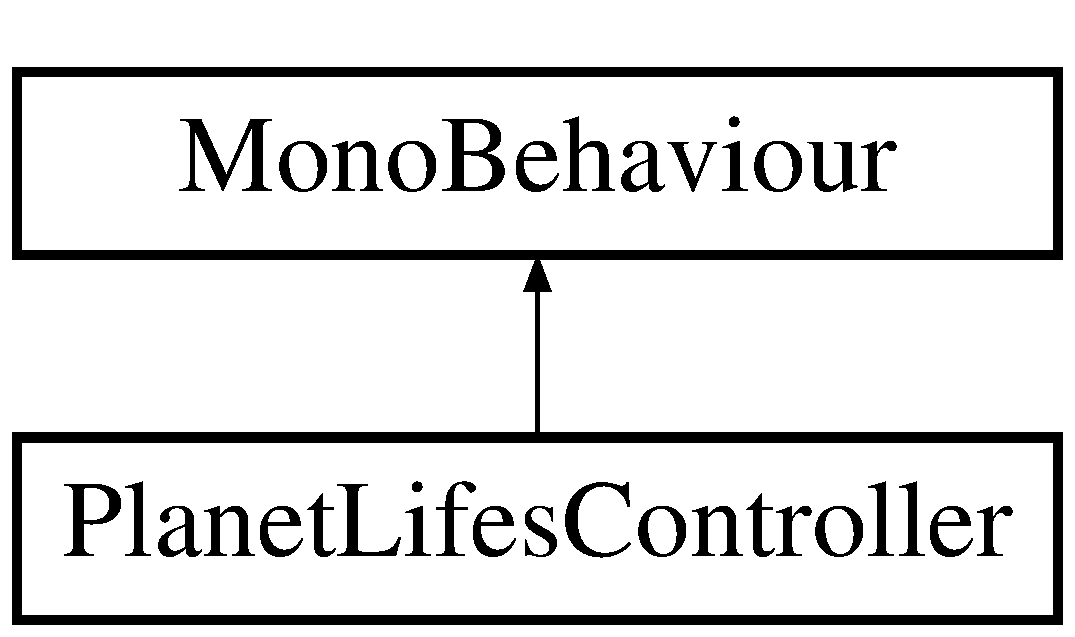
\includegraphics[height=2.000000cm]{class_planet_lifes_controller}
\end{center}
\end{figure}
\subsection*{Public Member Functions}
\begin{DoxyCompactItemize}
\item 
void \mbox{\hyperlink{class_planet_lifes_controller_acb812ee09ae6ed65b85baf971a582b25}{Start}} ()
\begin{DoxyCompactList}\small\item\em Initialization method. Sets main camera object and planet lifes. \end{DoxyCompactList}\item 
void \mbox{\hyperlink{class_planet_lifes_controller_a5f701b24bb0d90d38d049dec137f90b5}{On\+Collision\+Enter}} (Collision col)
\begin{DoxyCompactList}\small\item\em Checks if planet collides with bullets. \end{DoxyCompactList}\item 
void \mbox{\hyperlink{class_planet_lifes_controller_af81b69ec4a2d059ebd24bff38031a466}{decrement\+Lifes}} ()
\begin{DoxyCompactList}\small\item\em Decrements planet\textquotesingle{}s lifes and creates explosion object if planet is destroyed. \end{DoxyCompactList}\end{DoxyCompactItemize}
\subsection*{Public Attributes}
\begin{DoxyCompactItemize}
\item 
Game\+Object \mbox{\hyperlink{class_planet_lifes_controller_a793b98df14aca219bbdeec8fa0a21688}{explosion\+Effect}}
\begin{DoxyCompactList}\small\item\em Game\+Object representing the explossion efect. \end{DoxyCompactList}\end{DoxyCompactItemize}


\subsection{Detailed Description}
Class to control planet lifes and show explosion effect after it dies. 



\subsection{Member Function Documentation}
\mbox{\Hypertarget{class_planet_lifes_controller_af81b69ec4a2d059ebd24bff38031a466}\label{class_planet_lifes_controller_af81b69ec4a2d059ebd24bff38031a466}} 
\index{Planet\+Lifes\+Controller@{Planet\+Lifes\+Controller}!decrement\+Lifes@{decrement\+Lifes}}
\index{decrement\+Lifes@{decrement\+Lifes}!Planet\+Lifes\+Controller@{Planet\+Lifes\+Controller}}
\subsubsection{\texorpdfstring{decrement\+Lifes()}{decrementLifes()}}
{\footnotesize\ttfamily void Planet\+Lifes\+Controller.\+decrement\+Lifes (\begin{DoxyParamCaption}{ }\end{DoxyParamCaption})}



Decrements planet\textquotesingle{}s lifes and creates explosion object if planet is destroyed. 

\mbox{\Hypertarget{class_planet_lifes_controller_a5f701b24bb0d90d38d049dec137f90b5}\label{class_planet_lifes_controller_a5f701b24bb0d90d38d049dec137f90b5}} 
\index{Planet\+Lifes\+Controller@{Planet\+Lifes\+Controller}!On\+Collision\+Enter@{On\+Collision\+Enter}}
\index{On\+Collision\+Enter@{On\+Collision\+Enter}!Planet\+Lifes\+Controller@{Planet\+Lifes\+Controller}}
\subsubsection{\texorpdfstring{On\+Collision\+Enter()}{OnCollisionEnter()}}
{\footnotesize\ttfamily void Planet\+Lifes\+Controller.\+On\+Collision\+Enter (\begin{DoxyParamCaption}\item[{Collision}]{col }\end{DoxyParamCaption})}



Checks if planet collides with bullets. 

\mbox{\Hypertarget{class_planet_lifes_controller_acb812ee09ae6ed65b85baf971a582b25}\label{class_planet_lifes_controller_acb812ee09ae6ed65b85baf971a582b25}} 
\index{Planet\+Lifes\+Controller@{Planet\+Lifes\+Controller}!Start@{Start}}
\index{Start@{Start}!Planet\+Lifes\+Controller@{Planet\+Lifes\+Controller}}
\subsubsection{\texorpdfstring{Start()}{Start()}}
{\footnotesize\ttfamily void Planet\+Lifes\+Controller.\+Start (\begin{DoxyParamCaption}{ }\end{DoxyParamCaption})}



Initialization method. Sets main camera object and planet lifes. 



\subsection{Member Data Documentation}
\mbox{\Hypertarget{class_planet_lifes_controller_a793b98df14aca219bbdeec8fa0a21688}\label{class_planet_lifes_controller_a793b98df14aca219bbdeec8fa0a21688}} 
\index{Planet\+Lifes\+Controller@{Planet\+Lifes\+Controller}!explosion\+Effect@{explosion\+Effect}}
\index{explosion\+Effect@{explosion\+Effect}!Planet\+Lifes\+Controller@{Planet\+Lifes\+Controller}}
\subsubsection{\texorpdfstring{explosion\+Effect}{explosionEffect}}
{\footnotesize\ttfamily Game\+Object Planet\+Lifes\+Controller.\+explosion\+Effect}



Game\+Object representing the explossion efect. 



The documentation for this class was generated from the following file\+:\begin{DoxyCompactItemize}
\item 
Planet\+Lifes\+Controller.\+cs\end{DoxyCompactItemize}

\hypertarget{class_play_again}{}\section{Play\+Again Class Reference}
\label{class_play_again}\index{Play\+Again@{Play\+Again}}


Class responsible for playing the scene again.  


Inheritance diagram for Play\+Again\+:\begin{figure}[H]
\begin{center}
\leavevmode
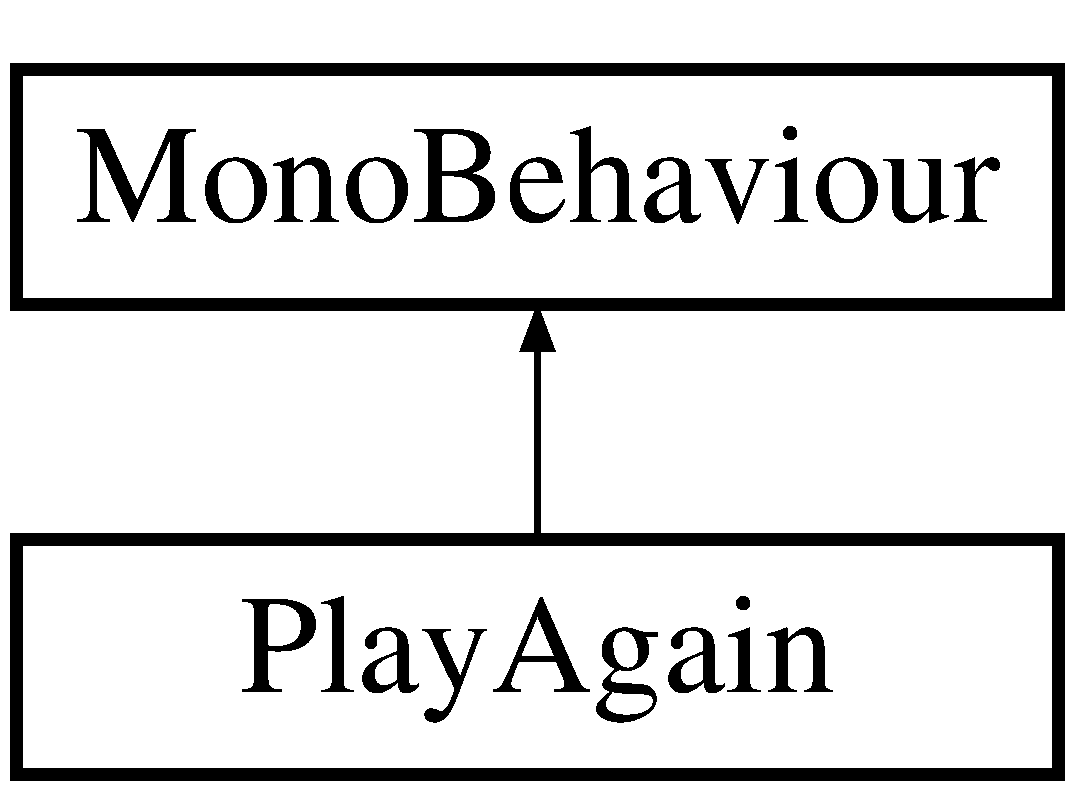
\includegraphics[height=2.000000cm]{class_play_again}
\end{center}
\end{figure}
\subsection*{Public Member Functions}
\begin{DoxyCompactItemize}
\item 
void \mbox{\hyperlink{class_play_again_af43857b80384f4ef6ef3bda6e8ac525c}{Start\+Level}} (int level)
\begin{DoxyCompactList}\small\item\em Starts the same level again. \end{DoxyCompactList}\end{DoxyCompactItemize}
\subsection*{Public Attributes}
\begin{DoxyCompactItemize}
\item 
Transform \mbox{\hyperlink{class_play_again_ad48a4dfa626a86c3b686a6c66537612e}{canvas}}
\begin{DoxyCompactList}\small\item\em \char`\"{}\+Game over\char`\"{} canvas. \end{DoxyCompactList}\end{DoxyCompactItemize}


\subsection{Detailed Description}
Class responsible for playing the scene again. 



\subsection{Member Function Documentation}
\mbox{\Hypertarget{class_play_again_af43857b80384f4ef6ef3bda6e8ac525c}\label{class_play_again_af43857b80384f4ef6ef3bda6e8ac525c}} 
\index{Play\+Again@{Play\+Again}!Start\+Level@{Start\+Level}}
\index{Start\+Level@{Start\+Level}!Play\+Again@{Play\+Again}}
\subsubsection{\texorpdfstring{Start\+Level()}{StartLevel()}}
{\footnotesize\ttfamily void Play\+Again.\+Start\+Level (\begin{DoxyParamCaption}\item[{int}]{level }\end{DoxyParamCaption})}



Starts the same level again. 


\begin{DoxyParams}{Parameters}
{\em level} & Level to play.\\
\hline
\end{DoxyParams}


\subsection{Member Data Documentation}
\mbox{\Hypertarget{class_play_again_ad48a4dfa626a86c3b686a6c66537612e}\label{class_play_again_ad48a4dfa626a86c3b686a6c66537612e}} 
\index{Play\+Again@{Play\+Again}!canvas@{canvas}}
\index{canvas@{canvas}!Play\+Again@{Play\+Again}}
\subsubsection{\texorpdfstring{canvas}{canvas}}
{\footnotesize\ttfamily Transform Play\+Again.\+canvas}



\char`\"{}\+Game over\char`\"{} canvas. 



The documentation for this class was generated from the following file\+:\begin{DoxyCompactItemize}
\item 
menus/Play\+Again.\+cs\end{DoxyCompactItemize}

\hypertarget{class_player_attributes}{}\section{Player\+Attributes Class Reference}
\label{class_player_attributes}\index{Player\+Attributes@{Player\+Attributes}}


Player attributes, like speed, rate of fire, ...  


Inheritance diagram for Player\+Attributes\+:\begin{figure}[H]
\begin{center}
\leavevmode
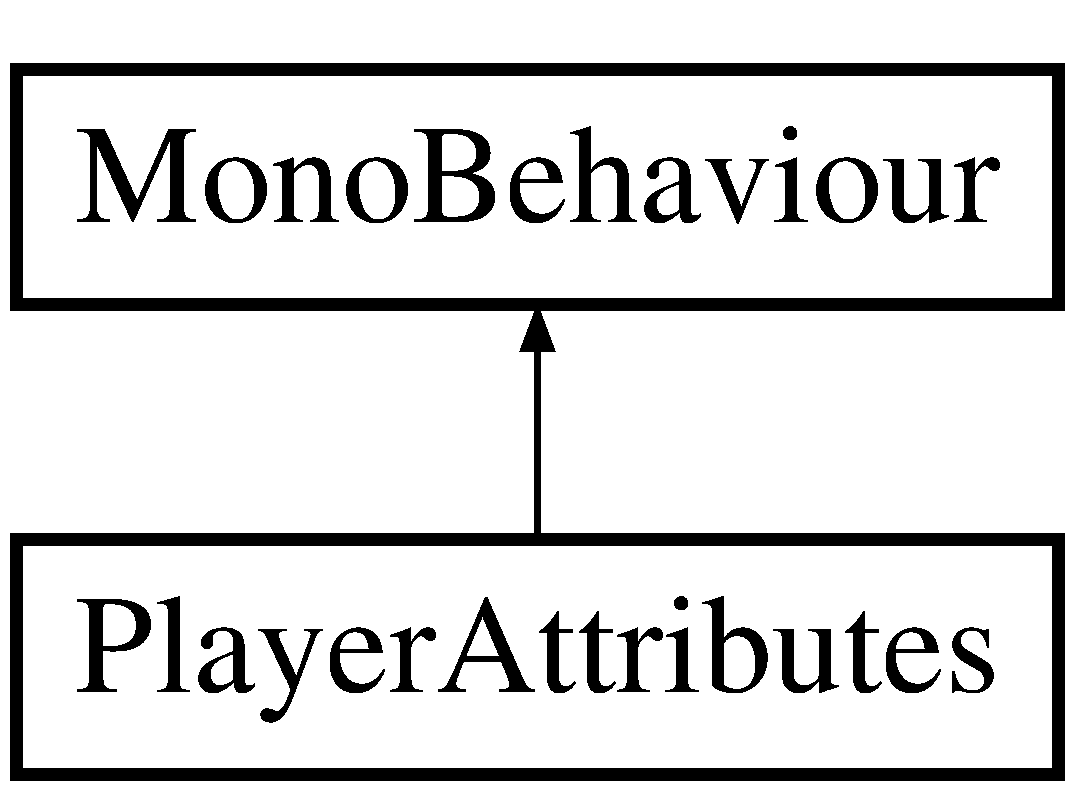
\includegraphics[height=2.000000cm]{class_player_attributes}
\end{center}
\end{figure}
\subsection*{Public Member Functions}
\begin{DoxyCompactItemize}
\item 
void \mbox{\hyperlink{class_player_attributes_ae04bfec3ffddefb521aca753c9b832ea}{Decrement\+Lives}} ()
\begin{DoxyCompactList}\small\item\em Decrements the lives and update the text manager \end{DoxyCompactList}\item 
void \mbox{\hyperlink{class_player_attributes_a0dfec30b6ea5d4246790c1038c6e4c45}{Increment\+Lives}} ()
\begin{DoxyCompactList}\small\item\em Increments the lives and update the text manager \end{DoxyCompactList}\end{DoxyCompactItemize}
\subsection*{Public Attributes}
\begin{DoxyCompactItemize}
\item 
int \mbox{\hyperlink{class_player_attributes_aa666ed9677fdae99cca2a98ab6796ea7}{lives}}
\begin{DoxyCompactList}\small\item\em The lives. \end{DoxyCompactList}\item 
bool \mbox{\hyperlink{class_player_attributes_a4bb2a3a44344d0e8e05ffd3c02b5e66c}{is\+Fire}}
\begin{DoxyCompactList}\small\item\em The is fire. \end{DoxyCompactList}\item 
float \mbox{\hyperlink{class_player_attributes_a8635c9f8b5b38f06899752f7df80a65b}{rate\+Of\+Fire}}
\begin{DoxyCompactList}\small\item\em The rate of fire. \end{DoxyCompactList}\item 
float \mbox{\hyperlink{class_player_attributes_a3c05ed20ca014ddef39d9e361bf9afe9}{speed}}
\begin{DoxyCompactList}\small\item\em The speed. \end{DoxyCompactList}\item 
bool \mbox{\hyperlink{class_player_attributes_a0b731fb2d368a90acfeaf37692bd1e33}{is\+Super\+Speed}} = false
\begin{DoxyCompactList}\small\item\em The is super speed. \end{DoxyCompactList}\item 
float \mbox{\hyperlink{class_player_attributes_a8d65a1b221e07cde721025345011066f}{super\+Speed\+Time}}
\begin{DoxyCompactList}\small\item\em The super speed time. \end{DoxyCompactList}\end{DoxyCompactItemize}
\subsection*{Private Member Functions}
\begin{DoxyCompactItemize}
\item 
void \mbox{\hyperlink{class_player_attributes_afa03395e71444c6bbaa339236b13ff64}{Start}} ()
\begin{DoxyCompactList}\small\item\em Sets starting values. \end{DoxyCompactList}\item 
void \mbox{\hyperlink{class_player_attributes_a9c30141dd1440bd1495b69b0f261190c}{set\+Player\+Position}} ()
\begin{DoxyCompactList}\small\item\em Sets player starting position (near screen width ends). \end{DoxyCompactList}\item 
void \mbox{\hyperlink{class_player_attributes_a5b1eb70086158522067e99f7900b679c}{Update}} ()
\begin{DoxyCompactList}\small\item\em Chcecks if super speed bonus is activated -\/ if so, rate of fire will be smaller. \end{DoxyCompactList}\item 
void \mbox{\hyperlink{class_player_attributes_a536939a7d2aedf70cfc7a2359ac1784f}{change\+Rate\+Of\+Fire}} ()
\begin{DoxyCompactList}\small\item\em Makes rate of fire smaller -\/ equal to 0, if real player is playing ad equal to 0.\+2, if it is \mbox{\hyperlink{class_a_i_enemy}{A\+I\+Enemy}}. After some time, all should go back to normal. \end{DoxyCompactList}\end{DoxyCompactItemize}
\subsection*{Private Attributes}
\begin{DoxyCompactItemize}
\item 
float \mbox{\hyperlink{class_player_attributes_a50bc8cd57496e1cea3634400aeda3e6f}{super\+Speed\+Left\+Time}}
\begin{DoxyCompactList}\small\item\em The super speed left time. \end{DoxyCompactList}\item 
float \mbox{\hyperlink{class_player_attributes_a15db75878d8d850cf083ff6a35751fd3}{typical\+Rate\+Of\+Fire}}
\begin{DoxyCompactList}\small\item\em The typical speed time. \end{DoxyCompactList}\item 
const string \mbox{\hyperlink{class_player_attributes_ada16579515985aa8211ab7ab641d7fd1}{enemy\+Tag}} = \char`\"{}Enemy\char`\"{}
\begin{DoxyCompactList}\small\item\em The tag of the enemy. \end{DoxyCompactList}\item 
const int \mbox{\hyperlink{class_player_attributes_a12ebc8e85046ee0c599280cd249c5c85}{move\+Away\+Distance}} = 3
\begin{DoxyCompactList}\small\item\em How far from the edge of the screen will be player placed. \end{DoxyCompactList}\item 
const float \mbox{\hyperlink{class_player_attributes_a76695d1cf2e07103e9efb4cdbdc17672}{super\+Speed\+Player\+Rate\+Of\+Fire}} = 0
\begin{DoxyCompactList}\small\item\em The rate of fire that the player will get in super speed mode. \end{DoxyCompactList}\item 
const float \mbox{\hyperlink{class_player_attributes_a734f84c1f66f934ab934e1314c9cd48f}{super\+Speed\+A\+I\+Enemy\+Rate\+Of\+Fire}} = 0.\+2f
\begin{DoxyCompactList}\small\item\em The rate of fire that the AI enemy will get in super speed mode. \end{DoxyCompactList}\end{DoxyCompactItemize}


\subsection{Detailed Description}
Player attributes, like speed, rate of fire, ... 



\subsection{Member Function Documentation}
\mbox{\Hypertarget{class_player_attributes_a536939a7d2aedf70cfc7a2359ac1784f}\label{class_player_attributes_a536939a7d2aedf70cfc7a2359ac1784f}} 
\index{Player\+Attributes@{Player\+Attributes}!change\+Rate\+Of\+Fire@{change\+Rate\+Of\+Fire}}
\index{change\+Rate\+Of\+Fire@{change\+Rate\+Of\+Fire}!Player\+Attributes@{Player\+Attributes}}
\subsubsection{\texorpdfstring{change\+Rate\+Of\+Fire()}{changeRateOfFire()}}
{\footnotesize\ttfamily void Player\+Attributes.\+change\+Rate\+Of\+Fire (\begin{DoxyParamCaption}{ }\end{DoxyParamCaption})\hspace{0.3cm}{\ttfamily [private]}}



Makes rate of fire smaller -\/ equal to 0, if real player is playing ad equal to 0.\+2, if it is \mbox{\hyperlink{class_a_i_enemy}{A\+I\+Enemy}}. After some time, all should go back to normal. 

\mbox{\Hypertarget{class_player_attributes_ae04bfec3ffddefb521aca753c9b832ea}\label{class_player_attributes_ae04bfec3ffddefb521aca753c9b832ea}} 
\index{Player\+Attributes@{Player\+Attributes}!Decrement\+Lives@{Decrement\+Lives}}
\index{Decrement\+Lives@{Decrement\+Lives}!Player\+Attributes@{Player\+Attributes}}
\subsubsection{\texorpdfstring{Decrement\+Lives()}{DecrementLives()}}
{\footnotesize\ttfamily void Player\+Attributes.\+Decrement\+Lives (\begin{DoxyParamCaption}{ }\end{DoxyParamCaption})}



Decrements the lives and update the text manager 

\mbox{\Hypertarget{class_player_attributes_a0dfec30b6ea5d4246790c1038c6e4c45}\label{class_player_attributes_a0dfec30b6ea5d4246790c1038c6e4c45}} 
\index{Player\+Attributes@{Player\+Attributes}!Increment\+Lives@{Increment\+Lives}}
\index{Increment\+Lives@{Increment\+Lives}!Player\+Attributes@{Player\+Attributes}}
\subsubsection{\texorpdfstring{Increment\+Lives()}{IncrementLives()}}
{\footnotesize\ttfamily void Player\+Attributes.\+Increment\+Lives (\begin{DoxyParamCaption}{ }\end{DoxyParamCaption})}



Increments the lives and update the text manager 

\mbox{\Hypertarget{class_player_attributes_a9c30141dd1440bd1495b69b0f261190c}\label{class_player_attributes_a9c30141dd1440bd1495b69b0f261190c}} 
\index{Player\+Attributes@{Player\+Attributes}!set\+Player\+Position@{set\+Player\+Position}}
\index{set\+Player\+Position@{set\+Player\+Position}!Player\+Attributes@{Player\+Attributes}}
\subsubsection{\texorpdfstring{set\+Player\+Position()}{setPlayerPosition()}}
{\footnotesize\ttfamily void Player\+Attributes.\+set\+Player\+Position (\begin{DoxyParamCaption}{ }\end{DoxyParamCaption})\hspace{0.3cm}{\ttfamily [private]}}



Sets player starting position (near screen width ends). 

\mbox{\Hypertarget{class_player_attributes_afa03395e71444c6bbaa339236b13ff64}\label{class_player_attributes_afa03395e71444c6bbaa339236b13ff64}} 
\index{Player\+Attributes@{Player\+Attributes}!Start@{Start}}
\index{Start@{Start}!Player\+Attributes@{Player\+Attributes}}
\subsubsection{\texorpdfstring{Start()}{Start()}}
{\footnotesize\ttfamily void Player\+Attributes.\+Start (\begin{DoxyParamCaption}{ }\end{DoxyParamCaption})\hspace{0.3cm}{\ttfamily [private]}}



Sets starting values. 

\mbox{\Hypertarget{class_player_attributes_a5b1eb70086158522067e99f7900b679c}\label{class_player_attributes_a5b1eb70086158522067e99f7900b679c}} 
\index{Player\+Attributes@{Player\+Attributes}!Update@{Update}}
\index{Update@{Update}!Player\+Attributes@{Player\+Attributes}}
\subsubsection{\texorpdfstring{Update()}{Update()}}
{\footnotesize\ttfamily void Player\+Attributes.\+Update (\begin{DoxyParamCaption}{ }\end{DoxyParamCaption})\hspace{0.3cm}{\ttfamily [private]}}



Chcecks if super speed bonus is activated -\/ if so, rate of fire will be smaller. 



\subsection{Member Data Documentation}
\mbox{\Hypertarget{class_player_attributes_ada16579515985aa8211ab7ab641d7fd1}\label{class_player_attributes_ada16579515985aa8211ab7ab641d7fd1}} 
\index{Player\+Attributes@{Player\+Attributes}!enemy\+Tag@{enemy\+Tag}}
\index{enemy\+Tag@{enemy\+Tag}!Player\+Attributes@{Player\+Attributes}}
\subsubsection{\texorpdfstring{enemy\+Tag}{enemyTag}}
{\footnotesize\ttfamily const string Player\+Attributes.\+enemy\+Tag = \char`\"{}Enemy\char`\"{}\hspace{0.3cm}{\ttfamily [private]}}



The tag of the enemy. 

\mbox{\Hypertarget{class_player_attributes_a4bb2a3a44344d0e8e05ffd3c02b5e66c}\label{class_player_attributes_a4bb2a3a44344d0e8e05ffd3c02b5e66c}} 
\index{Player\+Attributes@{Player\+Attributes}!is\+Fire@{is\+Fire}}
\index{is\+Fire@{is\+Fire}!Player\+Attributes@{Player\+Attributes}}
\subsubsection{\texorpdfstring{is\+Fire}{isFire}}
{\footnotesize\ttfamily bool Player\+Attributes.\+is\+Fire}



The is fire. 

\mbox{\Hypertarget{class_player_attributes_a0b731fb2d368a90acfeaf37692bd1e33}\label{class_player_attributes_a0b731fb2d368a90acfeaf37692bd1e33}} 
\index{Player\+Attributes@{Player\+Attributes}!is\+Super\+Speed@{is\+Super\+Speed}}
\index{is\+Super\+Speed@{is\+Super\+Speed}!Player\+Attributes@{Player\+Attributes}}
\subsubsection{\texorpdfstring{is\+Super\+Speed}{isSuperSpeed}}
{\footnotesize\ttfamily bool Player\+Attributes.\+is\+Super\+Speed = false}



The is super speed. 

\mbox{\Hypertarget{class_player_attributes_aa666ed9677fdae99cca2a98ab6796ea7}\label{class_player_attributes_aa666ed9677fdae99cca2a98ab6796ea7}} 
\index{Player\+Attributes@{Player\+Attributes}!lives@{lives}}
\index{lives@{lives}!Player\+Attributes@{Player\+Attributes}}
\subsubsection{\texorpdfstring{lives}{lives}}
{\footnotesize\ttfamily int Player\+Attributes.\+lives}



The lives. 

\mbox{\Hypertarget{class_player_attributes_a12ebc8e85046ee0c599280cd249c5c85}\label{class_player_attributes_a12ebc8e85046ee0c599280cd249c5c85}} 
\index{Player\+Attributes@{Player\+Attributes}!move\+Away\+Distance@{move\+Away\+Distance}}
\index{move\+Away\+Distance@{move\+Away\+Distance}!Player\+Attributes@{Player\+Attributes}}
\subsubsection{\texorpdfstring{move\+Away\+Distance}{moveAwayDistance}}
{\footnotesize\ttfamily const int Player\+Attributes.\+move\+Away\+Distance = 3\hspace{0.3cm}{\ttfamily [private]}}



How far from the edge of the screen will be player placed. 

\mbox{\Hypertarget{class_player_attributes_a8635c9f8b5b38f06899752f7df80a65b}\label{class_player_attributes_a8635c9f8b5b38f06899752f7df80a65b}} 
\index{Player\+Attributes@{Player\+Attributes}!rate\+Of\+Fire@{rate\+Of\+Fire}}
\index{rate\+Of\+Fire@{rate\+Of\+Fire}!Player\+Attributes@{Player\+Attributes}}
\subsubsection{\texorpdfstring{rate\+Of\+Fire}{rateOfFire}}
{\footnotesize\ttfamily float Player\+Attributes.\+rate\+Of\+Fire}



The rate of fire. 

\mbox{\Hypertarget{class_player_attributes_a3c05ed20ca014ddef39d9e361bf9afe9}\label{class_player_attributes_a3c05ed20ca014ddef39d9e361bf9afe9}} 
\index{Player\+Attributes@{Player\+Attributes}!speed@{speed}}
\index{speed@{speed}!Player\+Attributes@{Player\+Attributes}}
\subsubsection{\texorpdfstring{speed}{speed}}
{\footnotesize\ttfamily float Player\+Attributes.\+speed}



The speed. 

\mbox{\Hypertarget{class_player_attributes_a734f84c1f66f934ab934e1314c9cd48f}\label{class_player_attributes_a734f84c1f66f934ab934e1314c9cd48f}} 
\index{Player\+Attributes@{Player\+Attributes}!super\+Speed\+A\+I\+Enemy\+Rate\+Of\+Fire@{super\+Speed\+A\+I\+Enemy\+Rate\+Of\+Fire}}
\index{super\+Speed\+A\+I\+Enemy\+Rate\+Of\+Fire@{super\+Speed\+A\+I\+Enemy\+Rate\+Of\+Fire}!Player\+Attributes@{Player\+Attributes}}
\subsubsection{\texorpdfstring{super\+Speed\+A\+I\+Enemy\+Rate\+Of\+Fire}{superSpeedAIEnemyRateOfFire}}
{\footnotesize\ttfamily const float Player\+Attributes.\+super\+Speed\+A\+I\+Enemy\+Rate\+Of\+Fire = 0.\+2f\hspace{0.3cm}{\ttfamily [private]}}



The rate of fire that the AI enemy will get in super speed mode. 

\mbox{\Hypertarget{class_player_attributes_a50bc8cd57496e1cea3634400aeda3e6f}\label{class_player_attributes_a50bc8cd57496e1cea3634400aeda3e6f}} 
\index{Player\+Attributes@{Player\+Attributes}!super\+Speed\+Left\+Time@{super\+Speed\+Left\+Time}}
\index{super\+Speed\+Left\+Time@{super\+Speed\+Left\+Time}!Player\+Attributes@{Player\+Attributes}}
\subsubsection{\texorpdfstring{super\+Speed\+Left\+Time}{superSpeedLeftTime}}
{\footnotesize\ttfamily float Player\+Attributes.\+super\+Speed\+Left\+Time\hspace{0.3cm}{\ttfamily [private]}}



The super speed left time. 

\mbox{\Hypertarget{class_player_attributes_a76695d1cf2e07103e9efb4cdbdc17672}\label{class_player_attributes_a76695d1cf2e07103e9efb4cdbdc17672}} 
\index{Player\+Attributes@{Player\+Attributes}!super\+Speed\+Player\+Rate\+Of\+Fire@{super\+Speed\+Player\+Rate\+Of\+Fire}}
\index{super\+Speed\+Player\+Rate\+Of\+Fire@{super\+Speed\+Player\+Rate\+Of\+Fire}!Player\+Attributes@{Player\+Attributes}}
\subsubsection{\texorpdfstring{super\+Speed\+Player\+Rate\+Of\+Fire}{superSpeedPlayerRateOfFire}}
{\footnotesize\ttfamily const float Player\+Attributes.\+super\+Speed\+Player\+Rate\+Of\+Fire = 0\hspace{0.3cm}{\ttfamily [private]}}



The rate of fire that the player will get in super speed mode. 

\mbox{\Hypertarget{class_player_attributes_a8d65a1b221e07cde721025345011066f}\label{class_player_attributes_a8d65a1b221e07cde721025345011066f}} 
\index{Player\+Attributes@{Player\+Attributes}!super\+Speed\+Time@{super\+Speed\+Time}}
\index{super\+Speed\+Time@{super\+Speed\+Time}!Player\+Attributes@{Player\+Attributes}}
\subsubsection{\texorpdfstring{super\+Speed\+Time}{superSpeedTime}}
{\footnotesize\ttfamily float Player\+Attributes.\+super\+Speed\+Time}



The super speed time. 

\mbox{\Hypertarget{class_player_attributes_a15db75878d8d850cf083ff6a35751fd3}\label{class_player_attributes_a15db75878d8d850cf083ff6a35751fd3}} 
\index{Player\+Attributes@{Player\+Attributes}!typical\+Rate\+Of\+Fire@{typical\+Rate\+Of\+Fire}}
\index{typical\+Rate\+Of\+Fire@{typical\+Rate\+Of\+Fire}!Player\+Attributes@{Player\+Attributes}}
\subsubsection{\texorpdfstring{typical\+Rate\+Of\+Fire}{typicalRateOfFire}}
{\footnotesize\ttfamily float Player\+Attributes.\+typical\+Rate\+Of\+Fire\hspace{0.3cm}{\ttfamily [private]}}



The typical speed time. 



The documentation for this class was generated from the following file\+:\begin{DoxyCompactItemize}
\item 
Player/Player\+Attributes.\+cs\end{DoxyCompactItemize}

\hypertarget{class_player_chooser}{}\section{Player\+Chooser Class Reference}
\label{class_player_chooser}\index{Player\+Chooser@{Player\+Chooser}}


Class responsible for settig proper fields after user chooses playing mode (one or two players).  


Inheritance diagram for Player\+Chooser\+:\begin{figure}[H]
\begin{center}
\leavevmode
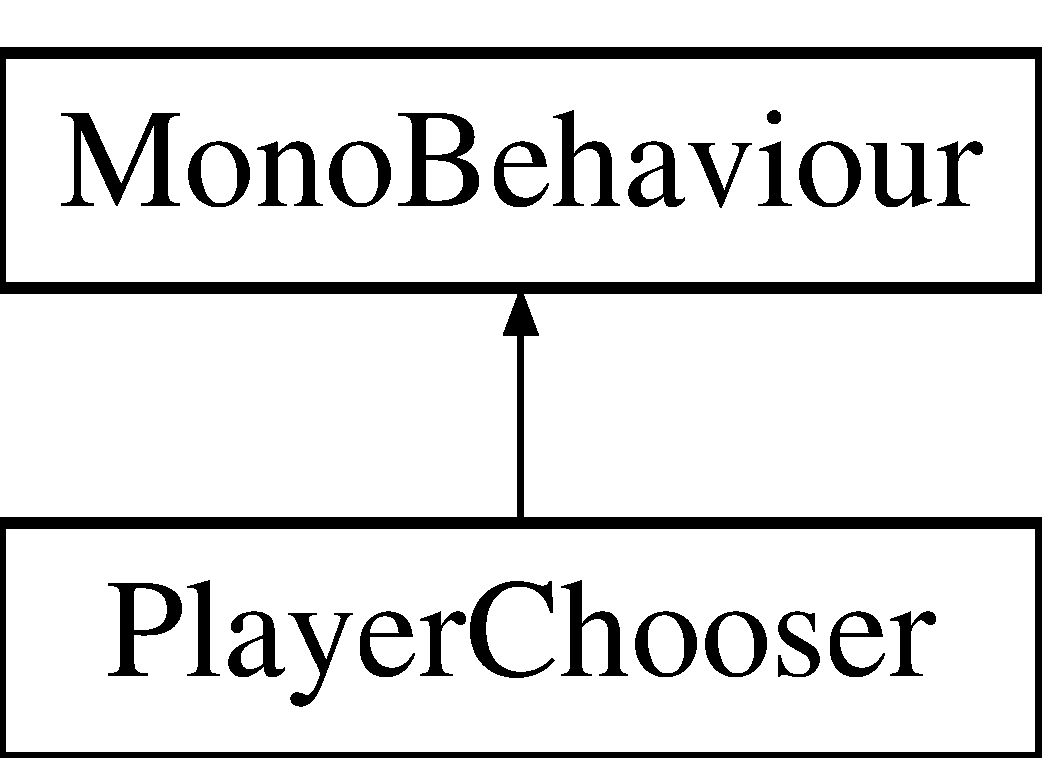
\includegraphics[height=2.000000cm]{class_player_chooser}
\end{center}
\end{figure}
\subsection*{Public Attributes}
\begin{DoxyCompactItemize}
\item 
Game\+Object \mbox{\hyperlink{class_player_chooser_a0b6190b6135c1cda958ac9d079a254c8}{player}}
\begin{DoxyCompactList}\small\item\em Player (enemy of main player). \end{DoxyCompactList}\end{DoxyCompactItemize}


\subsection{Detailed Description}
Class responsible for settig proper fields after user chooses playing mode (one or two players). 



\subsection{Member Data Documentation}
\mbox{\Hypertarget{class_player_chooser_a0b6190b6135c1cda958ac9d079a254c8}\label{class_player_chooser_a0b6190b6135c1cda958ac9d079a254c8}} 
\index{Player\+Chooser@{Player\+Chooser}!player@{player}}
\index{player@{player}!Player\+Chooser@{Player\+Chooser}}
\subsubsection{\texorpdfstring{player}{player}}
{\footnotesize\ttfamily Game\+Object Player\+Chooser.\+player}



Player (enemy of main player). 



The documentation for this class was generated from the following file\+:\begin{DoxyCompactItemize}
\item 
menus/Player\+Chooser.\+cs\end{DoxyCompactItemize}

\hypertarget{class_player_key_controller}{}\section{Player\+Key\+Controller Class Reference}
\label{class_player_key_controller}\index{Player\+Key\+Controller@{Player\+Key\+Controller}}


Player key controller, after pushing the button, update position of the player  


Inheritance diagram for Player\+Key\+Controller\+:\begin{figure}[H]
\begin{center}
\leavevmode
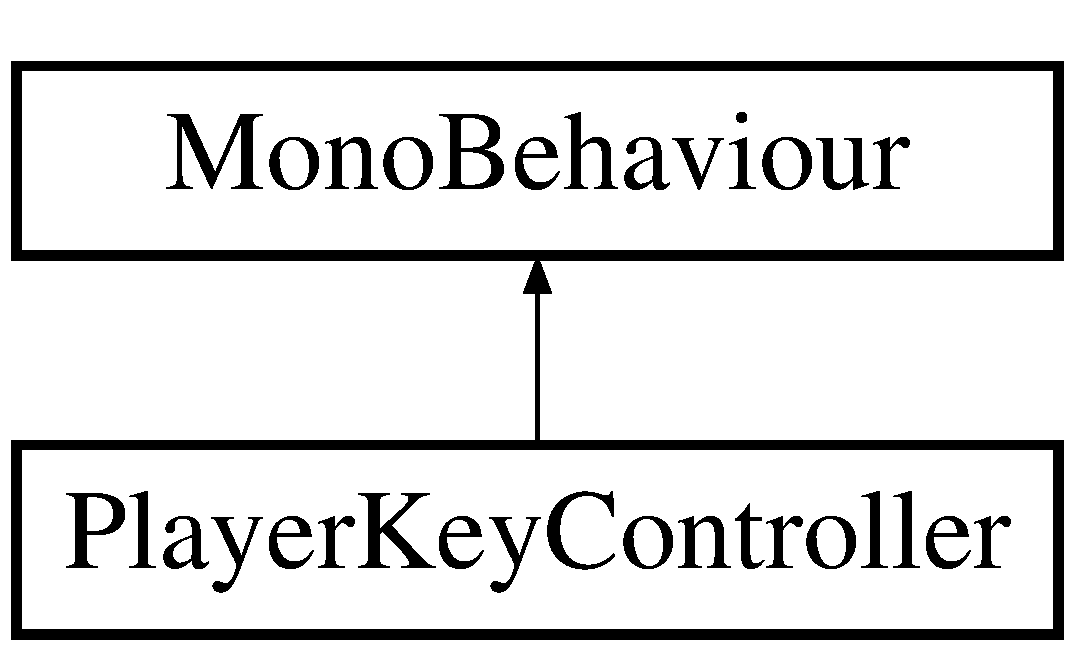
\includegraphics[height=2.000000cm]{class_player_key_controller}
\end{center}
\end{figure}
\subsection*{Public Attributes}
\begin{DoxyCompactItemize}
\item 
string \mbox{\hyperlink{class_player_key_controller_af6f283b7608be96f62f9af15b75c2691}{Vertical\+Key}}
\begin{DoxyCompactList}\small\item\em The vertical key. \end{DoxyCompactList}\item 
string \mbox{\hyperlink{class_player_key_controller_a0905f484ede4072fc87e2c7e46d45bed}{Horizontal\+Key}}
\begin{DoxyCompactList}\small\item\em The horizontal key. \end{DoxyCompactList}\end{DoxyCompactItemize}


\subsection{Detailed Description}
Player key controller, after pushing the button, update position of the player 



\subsection{Member Data Documentation}
\mbox{\Hypertarget{class_player_key_controller_a0905f484ede4072fc87e2c7e46d45bed}\label{class_player_key_controller_a0905f484ede4072fc87e2c7e46d45bed}} 
\index{Player\+Key\+Controller@{Player\+Key\+Controller}!Horizontal\+Key@{Horizontal\+Key}}
\index{Horizontal\+Key@{Horizontal\+Key}!Player\+Key\+Controller@{Player\+Key\+Controller}}
\subsubsection{\texorpdfstring{Horizontal\+Key}{HorizontalKey}}
{\footnotesize\ttfamily string Player\+Key\+Controller.\+Horizontal\+Key}



The horizontal key. 

\mbox{\Hypertarget{class_player_key_controller_af6f283b7608be96f62f9af15b75c2691}\label{class_player_key_controller_af6f283b7608be96f62f9af15b75c2691}} 
\index{Player\+Key\+Controller@{Player\+Key\+Controller}!Vertical\+Key@{Vertical\+Key}}
\index{Vertical\+Key@{Vertical\+Key}!Player\+Key\+Controller@{Player\+Key\+Controller}}
\subsubsection{\texorpdfstring{Vertical\+Key}{VerticalKey}}
{\footnotesize\ttfamily string Player\+Key\+Controller.\+Vertical\+Key}



The vertical key. 



The documentation for this class was generated from the following file\+:\begin{DoxyCompactItemize}
\item 
Player/Player\+Key\+Controller.\+cs\end{DoxyCompactItemize}

\hypertarget{class_quit_game}{}\section{Quit\+Game Class Reference}
\label{class_quit_game}\index{Quit\+Game@{Quit\+Game}}


Class responsible for quiting the game.  


Inheritance diagram for Quit\+Game\+:\begin{figure}[H]
\begin{center}
\leavevmode
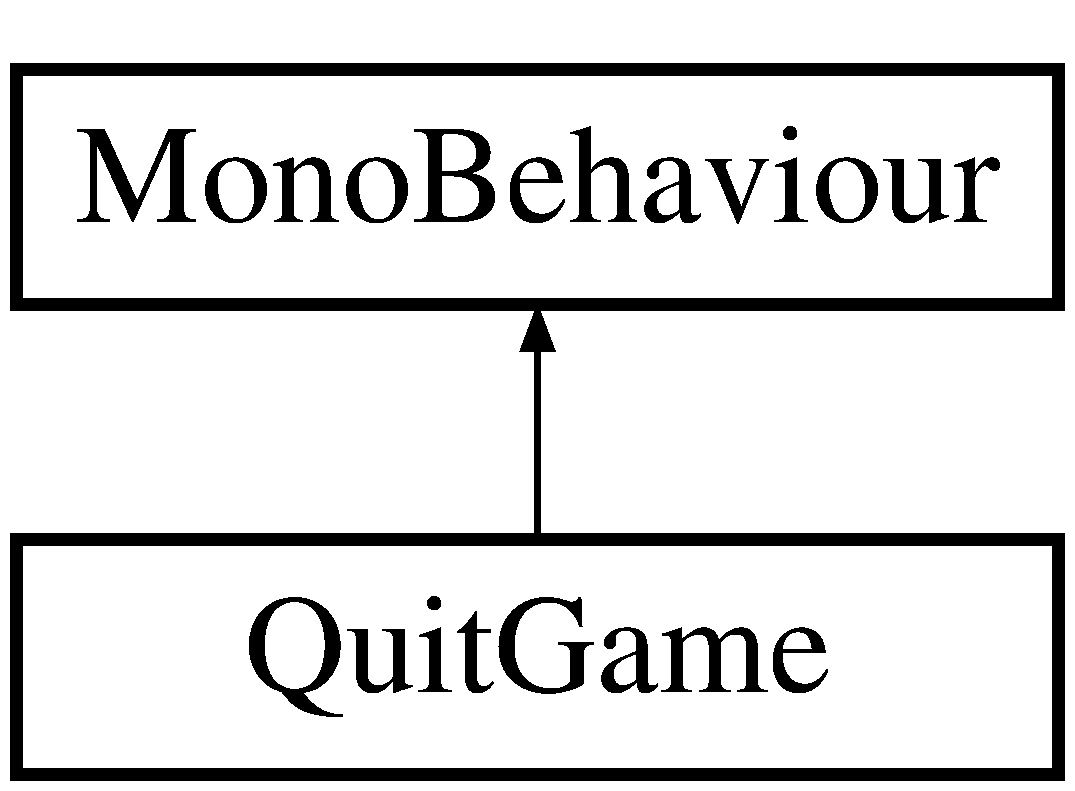
\includegraphics[height=2.000000cm]{class_quit_game}
\end{center}
\end{figure}
\subsection*{Public Member Functions}
\begin{DoxyCompactItemize}
\item 
void \mbox{\hyperlink{class_quit_game_ab91abbfccb620b7f99b0c661756d45e6}{quit\+Game}} ()
\begin{DoxyCompactList}\small\item\em Quits game. \end{DoxyCompactList}\end{DoxyCompactItemize}


\subsection{Detailed Description}
Class responsible for quiting the game. 



\subsection{Member Function Documentation}
\mbox{\Hypertarget{class_quit_game_ab91abbfccb620b7f99b0c661756d45e6}\label{class_quit_game_ab91abbfccb620b7f99b0c661756d45e6}} 
\index{Quit\+Game@{Quit\+Game}!quit\+Game@{quit\+Game}}
\index{quit\+Game@{quit\+Game}!Quit\+Game@{Quit\+Game}}
\subsubsection{\texorpdfstring{quit\+Game()}{quitGame()}}
{\footnotesize\ttfamily void Quit\+Game.\+quit\+Game (\begin{DoxyParamCaption}{ }\end{DoxyParamCaption})}



Quits game. 



The documentation for this class was generated from the following file\+:\begin{DoxyCompactItemize}
\item 
menus/Quit\+Game.\+cs\end{DoxyCompactItemize}

\hypertarget{classrotate}{}\section{rotate Class Reference}
\label{classrotate}\index{rotate@{rotate}}


Class responsible of rotation.  


Inheritance diagram for rotate\+:\begin{figure}[H]
\begin{center}
\leavevmode
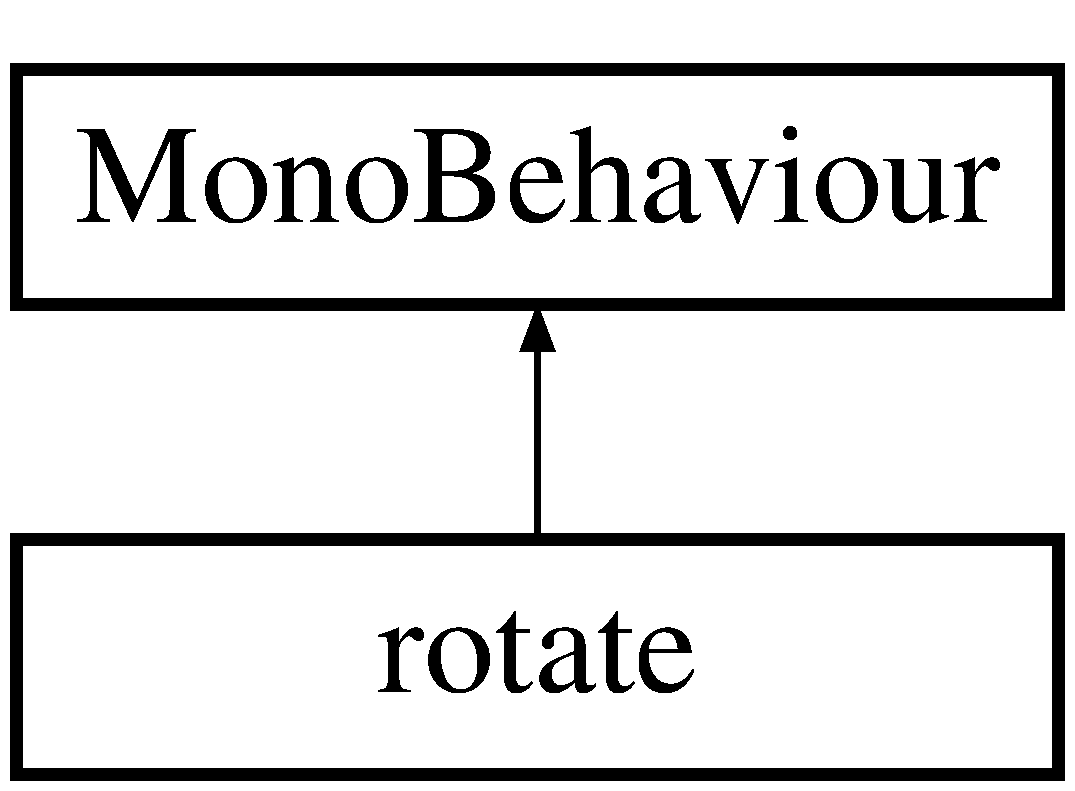
\includegraphics[height=2.000000cm]{classrotate}
\end{center}
\end{figure}
\subsection*{Public Attributes}
\begin{DoxyCompactItemize}
\item 
float \mbox{\hyperlink{classrotate_aad45a318094d5f91273252034e63b78b}{angle}} = 1
\begin{DoxyCompactList}\small\item\em Angle of rotation. \end{DoxyCompactList}\end{DoxyCompactItemize}


\subsection{Detailed Description}
Class responsible of rotation. 



\subsection{Member Data Documentation}
\mbox{\Hypertarget{classrotate_aad45a318094d5f91273252034e63b78b}\label{classrotate_aad45a318094d5f91273252034e63b78b}} 
\index{rotate@{rotate}!angle@{angle}}
\index{angle@{angle}!rotate@{rotate}}
\subsubsection{\texorpdfstring{angle}{angle}}
{\footnotesize\ttfamily float rotate.\+angle = 1}



Angle of rotation. 



The documentation for this class was generated from the following file\+:\begin{DoxyCompactItemize}
\item 
background tasks/rotate.\+cs\end{DoxyCompactItemize}

\hypertarget{class_start_playing_scene}{}\section{Start\+Playing\+Scene Class Reference}
\label{class_start_playing_scene}\index{Start\+Playing\+Scene@{Start\+Playing\+Scene}}


Class responsible for starting playing the game.  


Inheritance diagram for Start\+Playing\+Scene\+:\begin{figure}[H]
\begin{center}
\leavevmode
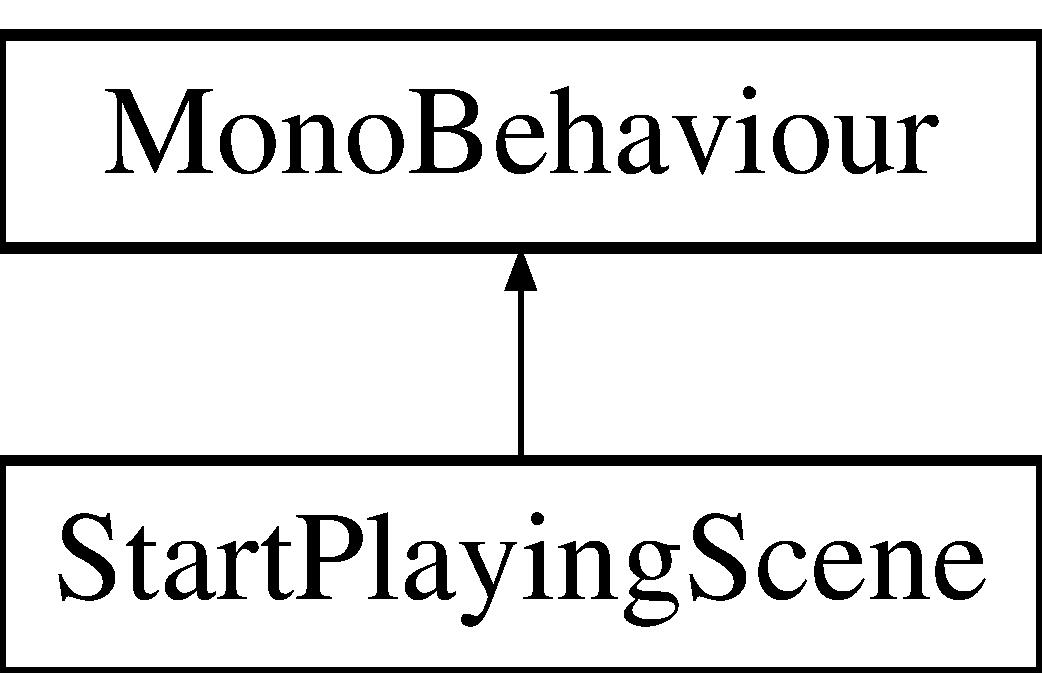
\includegraphics[height=2.000000cm]{class_start_playing_scene}
\end{center}
\end{figure}
\subsection*{Public Member Functions}
\begin{DoxyCompactItemize}
\item 
void \mbox{\hyperlink{class_start_playing_scene_a410c9893df6067ef27fb4fc2ce7f5394}{Start\+Level}} (int level)
\begin{DoxyCompactList}\small\item\em Starts playing the game. \end{DoxyCompactList}\end{DoxyCompactItemize}
\subsection*{Static Public Attributes}
\begin{DoxyCompactItemize}
\item 
static string \mbox{\hyperlink{class_start_playing_scene_aa349cb151f74693c91d971c2a6a20b26}{player\+Name}}
\begin{DoxyCompactList}\small\item\em Name of second player depending on playing mode (one or two players). \end{DoxyCompactList}\end{DoxyCompactItemize}


\subsection{Detailed Description}
Class responsible for starting playing the game. 



\subsection{Member Function Documentation}
\mbox{\Hypertarget{class_start_playing_scene_a410c9893df6067ef27fb4fc2ce7f5394}\label{class_start_playing_scene_a410c9893df6067ef27fb4fc2ce7f5394}} 
\index{Start\+Playing\+Scene@{Start\+Playing\+Scene}!Start\+Level@{Start\+Level}}
\index{Start\+Level@{Start\+Level}!Start\+Playing\+Scene@{Start\+Playing\+Scene}}
\subsubsection{\texorpdfstring{Start\+Level()}{StartLevel()}}
{\footnotesize\ttfamily void Start\+Playing\+Scene.\+Start\+Level (\begin{DoxyParamCaption}\item[{int}]{level }\end{DoxyParamCaption})}



Starts playing the game. 


\begin{DoxyParams}{Parameters}
{\em level} & Scene to play.\\
\hline
\end{DoxyParams}


\subsection{Member Data Documentation}
\mbox{\Hypertarget{class_start_playing_scene_aa349cb151f74693c91d971c2a6a20b26}\label{class_start_playing_scene_aa349cb151f74693c91d971c2a6a20b26}} 
\index{Start\+Playing\+Scene@{Start\+Playing\+Scene}!player\+Name@{player\+Name}}
\index{player\+Name@{player\+Name}!Start\+Playing\+Scene@{Start\+Playing\+Scene}}
\subsubsection{\texorpdfstring{player\+Name}{playerName}}
{\footnotesize\ttfamily string Start\+Playing\+Scene.\+player\+Name\hspace{0.3cm}{\ttfamily [static]}}



Name of second player depending on playing mode (one or two players). 



The documentation for this class was generated from the following file\+:\begin{DoxyCompactItemize}
\item 
menus/Start\+Playing\+Scene.\+cs\end{DoxyCompactItemize}

\hypertarget{class_text_manager}{}\section{Text\+Manager Class Reference}
\label{class_text_manager}\index{Text\+Manager@{Text\+Manager}}


Player\textquotesingle{}s text manu manager  


Inheritance diagram for Text\+Manager\+:\begin{figure}[H]
\begin{center}
\leavevmode
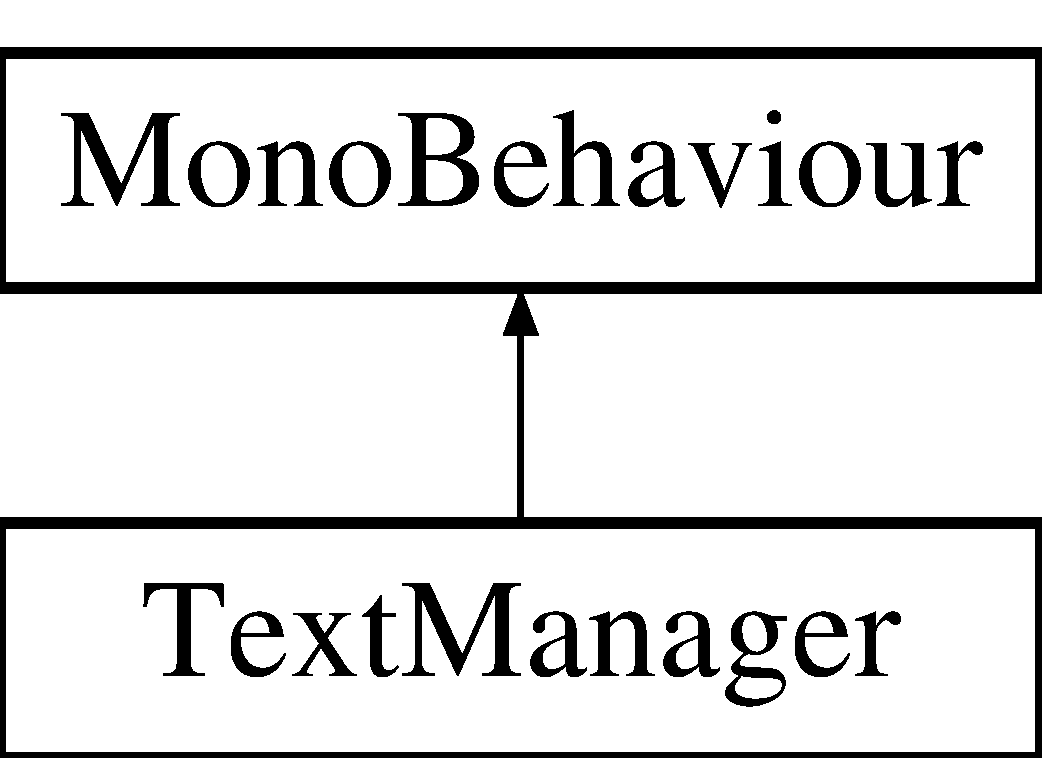
\includegraphics[height=2.000000cm]{class_text_manager}
\end{center}
\end{figure}
\subsection*{Public Member Functions}
\begin{DoxyCompactItemize}
\item 
void \mbox{\hyperlink{class_text_manager_a3bbadf652b27afb331e85866cc2b46d4}{Update\+Text\+Lives}} ()
\begin{DoxyCompactList}\small\item\em Updates the text lives. \end{DoxyCompactList}\end{DoxyCompactItemize}
\subsection*{Public Attributes}
\begin{DoxyCompactItemize}
\item 
Text \mbox{\hyperlink{class_text_manager_a8b12b74376f0b32cbef62f6b041e25f4}{text\+Lives}}
\begin{DoxyCompactList}\small\item\em Player lives text \end{DoxyCompactList}\end{DoxyCompactItemize}


\subsection{Detailed Description}
Player\textquotesingle{}s text manu manager 



\subsection{Member Function Documentation}
\mbox{\Hypertarget{class_text_manager_a3bbadf652b27afb331e85866cc2b46d4}\label{class_text_manager_a3bbadf652b27afb331e85866cc2b46d4}} 
\index{Text\+Manager@{Text\+Manager}!Update\+Text\+Lives@{Update\+Text\+Lives}}
\index{Update\+Text\+Lives@{Update\+Text\+Lives}!Text\+Manager@{Text\+Manager}}
\subsubsection{\texorpdfstring{Update\+Text\+Lives()}{UpdateTextLives()}}
{\footnotesize\ttfamily void Text\+Manager.\+Update\+Text\+Lives (\begin{DoxyParamCaption}{ }\end{DoxyParamCaption})}



Updates the text lives. 



\subsection{Member Data Documentation}
\mbox{\Hypertarget{class_text_manager_a8b12b74376f0b32cbef62f6b041e25f4}\label{class_text_manager_a8b12b74376f0b32cbef62f6b041e25f4}} 
\index{Text\+Manager@{Text\+Manager}!text\+Lives@{text\+Lives}}
\index{text\+Lives@{text\+Lives}!Text\+Manager@{Text\+Manager}}
\subsubsection{\texorpdfstring{text\+Lives}{textLives}}
{\footnotesize\ttfamily Text Text\+Manager.\+text\+Lives}



Player lives text 



The documentation for this class was generated from the following file\+:\begin{DoxyCompactItemize}
\item 
Player/Text\+Manager.\+cs\end{DoxyCompactItemize}

%--- End generated contents ---

% Index
\backmatter
\newpage
\phantomsection
\clearemptydoublepage
\addcontentsline{toc}{chapter}{Index}
\printindex

\end{document}
